\documentclass[10pt,twocolumn]{article}

% use the oxycomps style file
\usepackage{oxycomps}

% usage: \fixme[comments describing issue]{text to be fixed}
% define \fixme as not doing anything special
\newcommand{\fixme}[2][]{#2}
% overwrite it so it shows up as red
\renewcommand{\fixme}[2][]{\textcolor{red}{#2}}
% overwrite it again so related text shows as footnotes
%\renewcommand{\fixme}[2][]{\textcolor{red}{#2\footnote{#1}}}

% read references.bib for the bibtex data
\bibliography{references}

% include metadata in the generated pdf file
\pdfinfo{
    /Title (The Occidental Computer Science Comprehensive Project: Goals, Timeline, Format, and Advice)
    /Author (Justin Li)
}

% set the title and author information
\title{The Occidental Computer Science Comprehensive Project: \\ Computer Assembly Through Virtual Reality}
\author{Miriam Aguilar}
\affiliation{Occidental College}
\email{maguilar3@oxy.edu}

\begin{document}

\maketitle

\section{Introduction}

\par Building a personal computer (PC) is a popular alternative to purchasing one off the market. In some instances, choosing to purchase computer hardware and build it yourself costs less than purchasing an assembled computer. Furthermore, individuals tend to choose this option because it provides flexibility for the computer hardware \cite{Beltran2022BuildingYourOwn}. Individuals can customize the components to their liking, such as choosing higher-wattage power, better graphics, and/or increasing storage. 

\par Building a PC requires extensive preparation and research. Thus, individuals who have little to no familiarity with computer assembly may have difficulties knowing where to start with researching the process. The goal of this project is to demystify the computer assembly process by providing an immersive and interactive experience using virtual reality (VR). This VR platform specifically targets users who are unfamiliar with computer assembly and aims to teach them the basic assembly process. However, the platform is not exclusive to novice users, but is meant as a resource for any individual interested in the computer assembly process. Using the VR platform, users will interact with computer hardware and follow a sequence of steps to assemble a PC in a virtual reality environment. Users will gain practical skills and familiarity with PC hardware, ultimately bridging the gap between apprehension and competence in computer assembly. 

\section{Technical Background}

\subsection{VR Development}

\par There are multiple frameworks available for virtual reality development. Most of these frameworks share similarities in common workflow and design considerations with 3D development. This project specifically uses the Unity framework to deploy the 3D virtual environment. The Unity framework, equipped with the XR Interaction Toolkit, allows for deployment of VR projects to a supported head-mounted display (HMDs) and provides various components for developing interactions in VR \cite{Unity2023VRDevelopment}. Although there are many frameworks that work with VR, Unity has richer user input and 3D environment interactions. It also considers user comfort which makes it a preferable framework to use for virtual reality development \cite{Unity2023VRDevelopment}. The Unity framework also provides the XR Plug-in Management system which allows for support for most HMDs such as the Oculus, OpenXR, Playstation VR, and MOCK HDM \cite{Unity2023VRDevelopment}. This makes Unity an optimal framework for VR development.

\subsection{Virtual Reality Capabilities}

\subsubsection{User Input}

\par In Unity, the virtual reality interactions rely on an Input System. This package allows access to tracking data, haptics, and user input through the controller buttons \cite{Unity2023VRDevelopment}. The XR Controller prefabs in Unity also provide presets with basic interactions, such as grabbing an object. Using the data from the XR Controller, custom scripts specify the desired interactions between hardware objects and the user \cite{Valem2022HowToVR}. For example, a script can specify the user’s hand grab pose and position when grabbing an object [Figure 1]. 

\begin{figure}
    \centering
    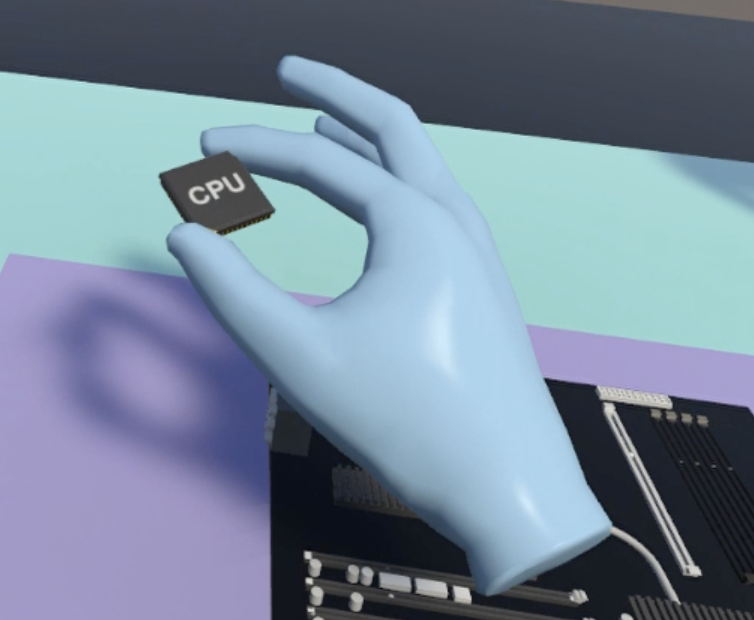
\includegraphics[width=2.4cm]{images/CPUCustomGrabPose.png}
    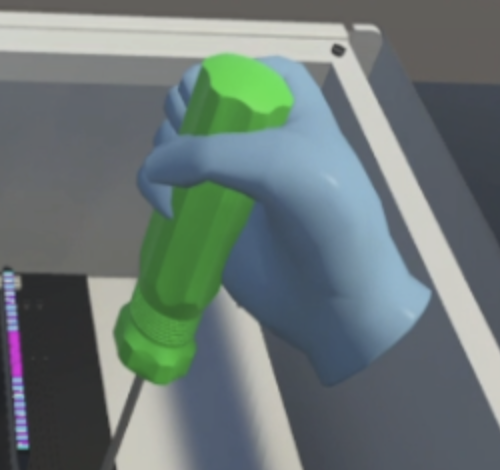
\includegraphics[width=2.1cm]{images/ScrewdriverCustomGrabPose.png}
    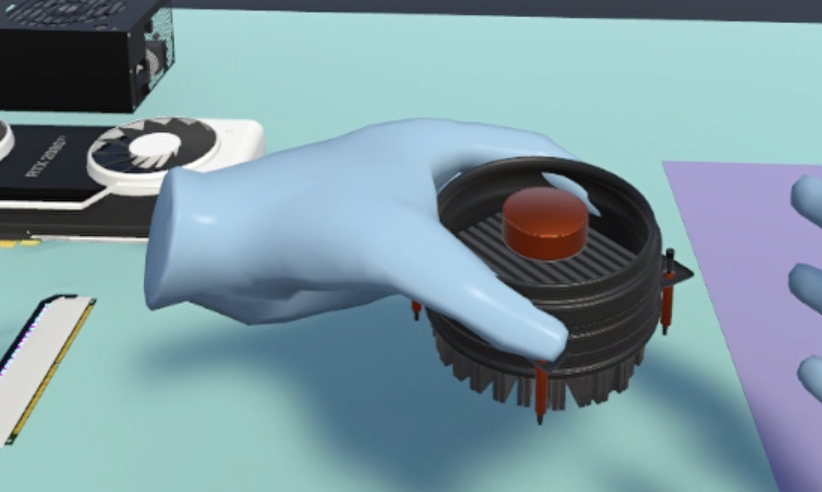
\includegraphics[width=3.3cm]{images/CoolerCustomGrabPose.png}
    \caption{CPU, Screwdriver, \& Cooler custom grab pose}
\end{figure}

\subsubsection{Objects}

\par The XR Interaction Toolkit also provides Interactor and Interactable components for objects. Components contain properties for each game object that define its behavior \cite{Unity2023IntroductionToComponents}. The Interactable objects allow for an Interactor to hover, select, and/or activate an object. Interactions can also be customized using these behaviors. For instance, certain actions trigger objects to adjust to a certain position, rotation, or scale \cite{Valem2022HowToVR}. Triggering these actions also allows for calls to custom script functions. Thus, using the Interactor \& Interactable components provide the option to define object behavior using custom scripts. 

\subsubsection{VR Scenes}

\par The Unity XR Interaction Toolkit provides an XR Origin for every scene in the project. The XR Origin defines the player’s 3D origin which is controlled by tracking data \cite{Unity2023VRDevelopment}. It also contains the Camera Offset, Main Camera, and Left and Right controllers. This collection of objects inside the XR Origin, allows for the user to move around and interact in the virtual environment \cite{Valem2022HowToVR}. This means the user can move around the world using the controller joysticks and grab objects using the controllers. The XR Origin can be adjusted depending on the level of interaction and movement you need for a scene. 

\subsection{Computer Assembly}

\par The computer assembly process requires extensive research and preparation. The instructions for assembling your computer may vary depending on the components you purchase. This platform focuses on a basic installation process for PC assembly. Before assembling your PC, it is vital to research hardware compatibility when choosing what components to purchase. For instance, an Intel CPU is compatible with an ASUS, MSI, Gigabyte, or ASRock motherboard \cite{Newegg2023IntelMotherboards}. It is important to consider compatibility to ensure all hardware is compatible prior to assembly. Due to the fragility of hardware components, the PC should not be powered throughout the assembly process and components should be handled with extreme caution and care. It is also necessary to have a clean space with room to work with all the components to avoid any damage to the hardware.

\begin{figure}
    \centering
    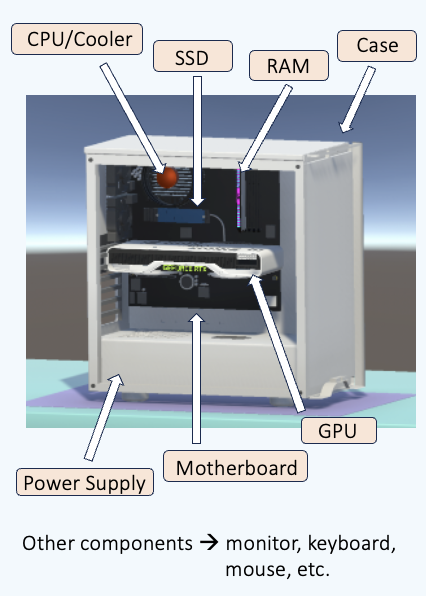
\includegraphics[width=7cm]{images/LabeledPC.png}
    \caption{A completed PC with the main hardware labeled.}
\end{figure}

\par The components required to build a PC are the following [Figure 2]: 

\begin{itemize}
    \item Central Processing Unit (CPU)
    \item Cooler Fan
    \item Random Access Memory (RAM)
    \item Solid State Drive (SSD)
    \item Graphics Processing Unit (GPU) 
    \item Motherboard 
    \item Case 
    \item Thermal Paste
    \item Power Supply Unit (PSU)
    \item Hard Drive (Optional)
    \item Screwdriver 
    \item Thermal Paste (May be pre-applied)    
\end{itemize}

\par Other recommended tools: 
\begin{itemize}
    \item Scissors
    \item Zip ties (For cable management)
    \item Anti-static mat
\end{itemize}

\par The Central Processing Unit (CPU) is the brain of the computer that processes all the information on a computational level [Figure 3]. It communicates with all other components and performs tasks required by the PC. There are many ways to attach a CPU to a motherboard \cite{Fisher2021EverythingYouNeed}.

\begin{figure}
    \centering
    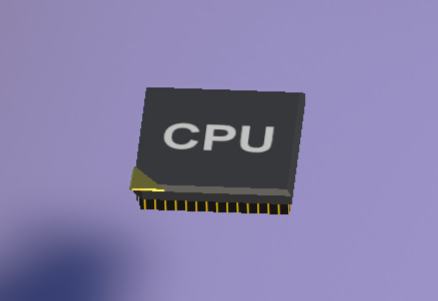
\includegraphics[width=5cm]{images/CPU1.png}
    \caption{The CPU object in the VR environment.}
\end{figure}

\begin{itemize}
    \item \textbf{Pin Grid Array (PGA):}  The CPU is attached to the socket using pins.
    \item \textbf{Land Grid Array (LGA):} A levered hinged plate clamps down the CPU to the motherboard. 
    \item \textbf{Ball Grid Array (BGA):} The CPU is soldered onto the motherboard. 
\end{itemize}

\par This project follows an Intel compatible assembly process. The CPU is installed using the LGA installation process which is the process used for most Intel CPUs \cite{GlobalAmerican2022TypesOfCPU}. It is vital to avoid touching the golden contact points on the CPU. For the LGA installation, the CPU is placed in the housing and then the latch is closed. This may require some force \cite{Sample2021HowToAssemble}. 

\par A CPU generates a decent amount of heat so a cooler is required to draw the heat away from the processor [Figure 4]. Many CPU coolers have pre-applied thermal paste. The thermal paste is a thermally conductive compound that is applied between the CPU and the heat sink of the cooler and allows for an efficient transfer of heat \cite{Intel2023HowToApply}. A Phillips head screwdriver is required to apply the cooler. First, line up the cooler over the CPU by aligning it over the screw holes on the motherboard. Then, secure the cooler by screwing in an X-shaped pattern to evenly tighten the screws \cite{Fisher2021EverythingYouNeed}. 

\par The Random Access Memory (RAM) is the volatile storage device, meaning that it loses data when the power is off [Figure 5]. The RAM plugs in directly to the RAM slot on the motherboard. Different RAMs may have different installation instructions \cite{Fisher2021EverythingYouNeed}. 

\par The Solid State Drive (SSD) is a non-volatile data storage device, meaning that it stores persistent data [Figure 6]. Depending on the motherboard, there should be contact points to connect the SSD to the motherboard. Plug in the SSD and secure its screw using the screwdriver \cite{Fisher2021EverythingYouNeed}. 

\begin{figure}
    \centering
    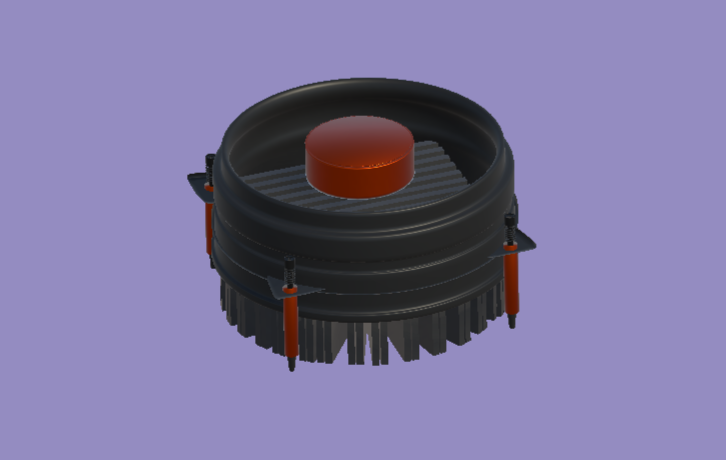
\includegraphics[width=5cm]{images/Cooler.png}
    \caption{The Cooler object in the VR environment.}
\end{figure}

\begin{figure}
    \centering
    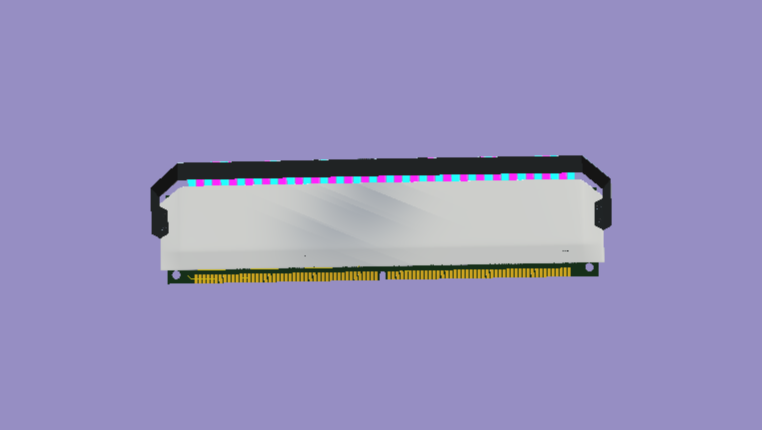
\includegraphics[width=5cm]{images/RAM.png}
    \caption{The RAM object in the VR environment.}
\end{figure}

\begin{figure}
    \centering
    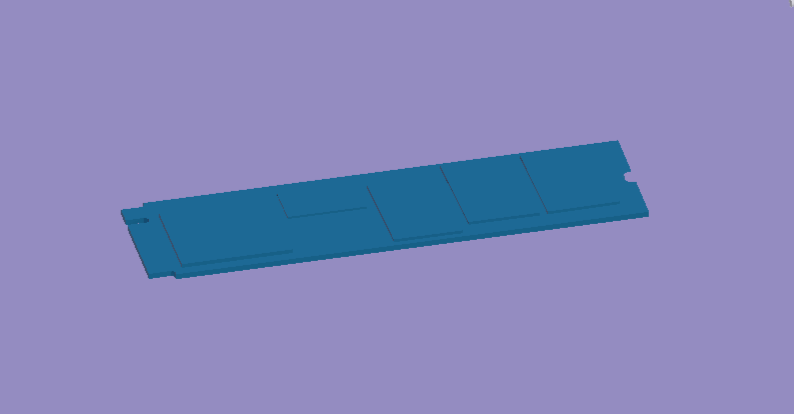
\includegraphics[width=5cm]{images/SSD.png}
    \caption{The SSD object in the VR environment.}
\end{figure}

\par Typically after installing these components, the motherboard is ready to be installed into the case. The motherboard is the circuit board that holds and allows communication between the different components of a computer [Figure 7] \cite{Fisher2021EverythingYouNeed}. The case should have a noticeable place for the motherboard. The motherboard should line up with the screw holes on the case. After gently placing the motherboard in the case, secure the board using screws. Avoid screwing the motherboard too tightly to avoid damage. Once screwed in, the motherboard should budge in the case \cite{Sample2021HowToAssemble}. 

\begin{figure}
    \centering
    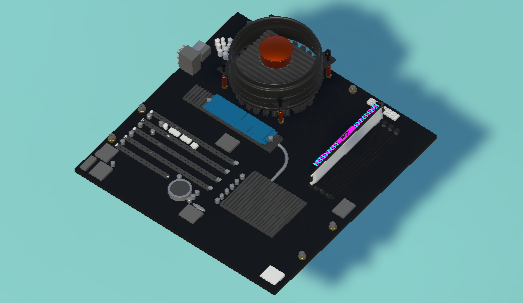
\includegraphics[width=5cm]{images/Motherboard.png}
    \caption{The Motherboard object in the VR environment.}
\end{figure}

\begin{figure}
    \centering
    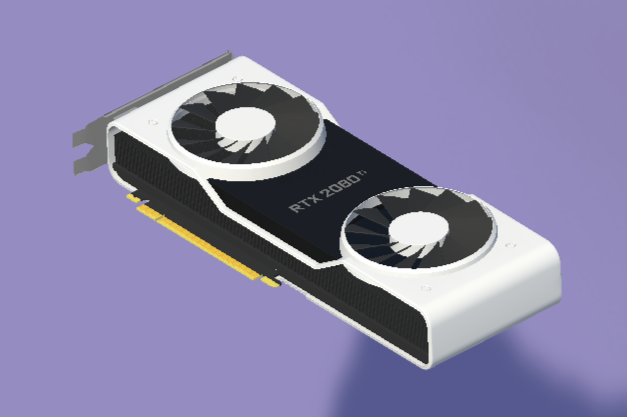
\includegraphics[width=5cm]{images/GPU.png}
    \caption{The GPU object in the VR environment.}
\end{figure}

\begin{figure}
    \centering
    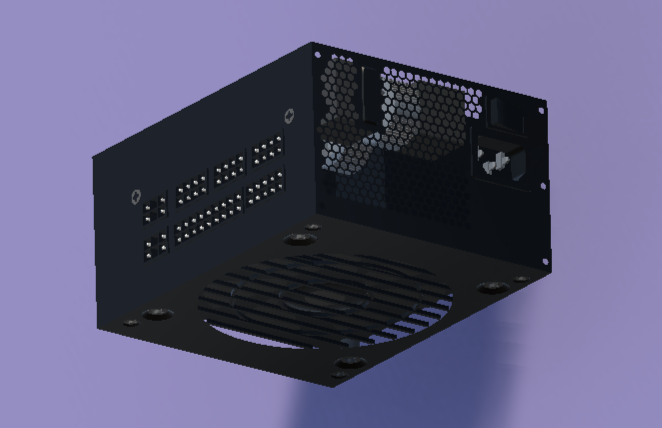
\includegraphics[width=5cm]{images/PowerSupply.png}
    \caption{The power supply object in the VR environment.}
\end{figure}

\par The Graphics Processing Unit (GPU) is a processor designed to accelerate graphics rendering [Figure 8] \cite{Fisher2021EverythingYouNeed}. To install the GPU, it is important to follow the steps for your specific type of GPU. Avoid touching the golden contact points on the GPU when aligning it with the corresponding slot on the motherboard. The GPU should be placed with little force and then secured using screws on the side panel of the case \cite{Sample2021HowToAssemble}. 

\par The Power Supply Unit (PSU) is the component that supplies power to the computer [Figure 9]. This installation step also varies depending on the type of PSU and the type of case. It is most common to place the PSU in the bottom of the case. The PSU fan should orient towards the outside of the case, then screw the PSU into place \cite{Sample2021HowToAssemble}. After installing the PSU, the connection cable should plug into the motherboard along with other connection cables (cooler, GPU, front panel, power, etc.). It is common for the outlets on the motherboard to have labels. Connect all the connections to their corresponding outlets on the motherboard \cite{Sample2021HowToAssemble}. After completing the PC build, connect your computer to a monitor, keyboard, and mouse. Then install the operating system for the computer. 

\section{Prior Work}

\par The computer assembly process relies heavily on instructional preparation. The goal of this platform is to use virtual reality technology as an additional resource for this instructional preparation. This platform is not meant to replace computer assembly research and preparation. Instead, the platform uses virtual reality’s unique elements to teach a complicated assembly task. In addition, VR’s physical and visual elements have shown to yield better results as an instructional medium \cite{Baird1999EvaluatingTheEffectiveness}. According to research on the effectiveness of reality technologies as instructional aids, reality technologies are more effective instructional aids for assembly tasks in comparison to paper and computer–aided instructions. The subjects in this study made fewer errors overall and had an increase in productivity \cite{Baird1999EvaluatingTheEffectiveness}. 

\par A study on the Motherboard Assembly Tutor(MAT) platform reveals the benefits of reality technology as instructional aids. MAT is a platform that aims to provide a more effective learning experience for users by delivering hands-on training using reality technologies \cite{Westerfield2015IntelligentAR}. MAT’s goal is to teach novice users how to assemble a computer motherboard using graphics in AR. MAT instructs tasks that are inherently spatial which makes reality technology’s hands-on interactions more natural and relevant to the assembly task. The results of user tests revealed an 82\% reduction in error rate for the instructed task. In addition, the study found that using HMDs increased the assembly speed of users by 52\% compared to paper instructions \cite{Westerfield2015IntelligentAR}. 

\par Physical and hands-on learning is beneficial in teaching an assembly task like computer assembly. The goal of the project is to emphasize the hardware installation steps using these physical motions. Thus, the benefits of reality technology make it an ideal technology to use for this project. The MAT study confirms that VR is a more beneficial medium for teaching a complicated process due to its ability to reduce errors for the user and increase user speed. Although speed is not a goal of this project, reality technologies show promising benefits in instructing assembly tasks like computer assembly. 

\par Virtual reality also contributes to an increase in user motivation. A study on educational VR platforms designed and developed the Virtual Reality Training System for Computer Hardware Assembly (VTSCHA). The VTSCHA platform aims to teach users computer hardware assembly using interactive content and real-time 3D animation \cite{Tong2020DesignAndApplication}. The platform incorporated an introduction interface, parts display, computer assembly demonstration, and a computer assembly simulation interface. The results from users testing revealed that VTSCHA has a positive teaching effect in the classroom. This is due to the nature of VR, which creates a sense of presence when learning by incorporating user physical interaction. Compared to traditional teaching methods, the study supports VR as a learning medium that contributes to increasing the curiosity of students learning computer assembly \cite{Chen2011AVirtualRealityExperiment}.

\par This platform considers that some users may new to computer assembly and learning the process for the first time. Increasing user motivation is an important factor in maintaining users engaged when learning an extensive and unfamiliar process. Thus, VR’s ability to increase user motivation using presence and physical motion makes it an beneficial platform to use to introduce the concept. 

\section{Methods}

\par The platform’s 3D virtual environment will have a simple setup. The environment will consist of a table and an anti-static mat [Figure 10]. This setup is where the user will interact with the components and assemble the PC. Each scene will have all the necessary components and tools laid out on the table. The overall assembly process will follow a step-by-step structure. In other words, the users will install the hardware following a fixed sequence of steps. The assembly process for this platform will follow the common sequence used in most instructional guides. 

\par The reason for using a step-by-step approach is that it provides more structure and guidance for a novice user. An alternative approach may allow for more freedom in the order that the user assembles the PC. However, a fixed structure is preferable for this project since users are not expected to be familiar with the common sequence for computer assembly. More guidance in the platform is preferred since most users will not have previous knowledge of computer assembly.

\begin{figure}
    \centering
    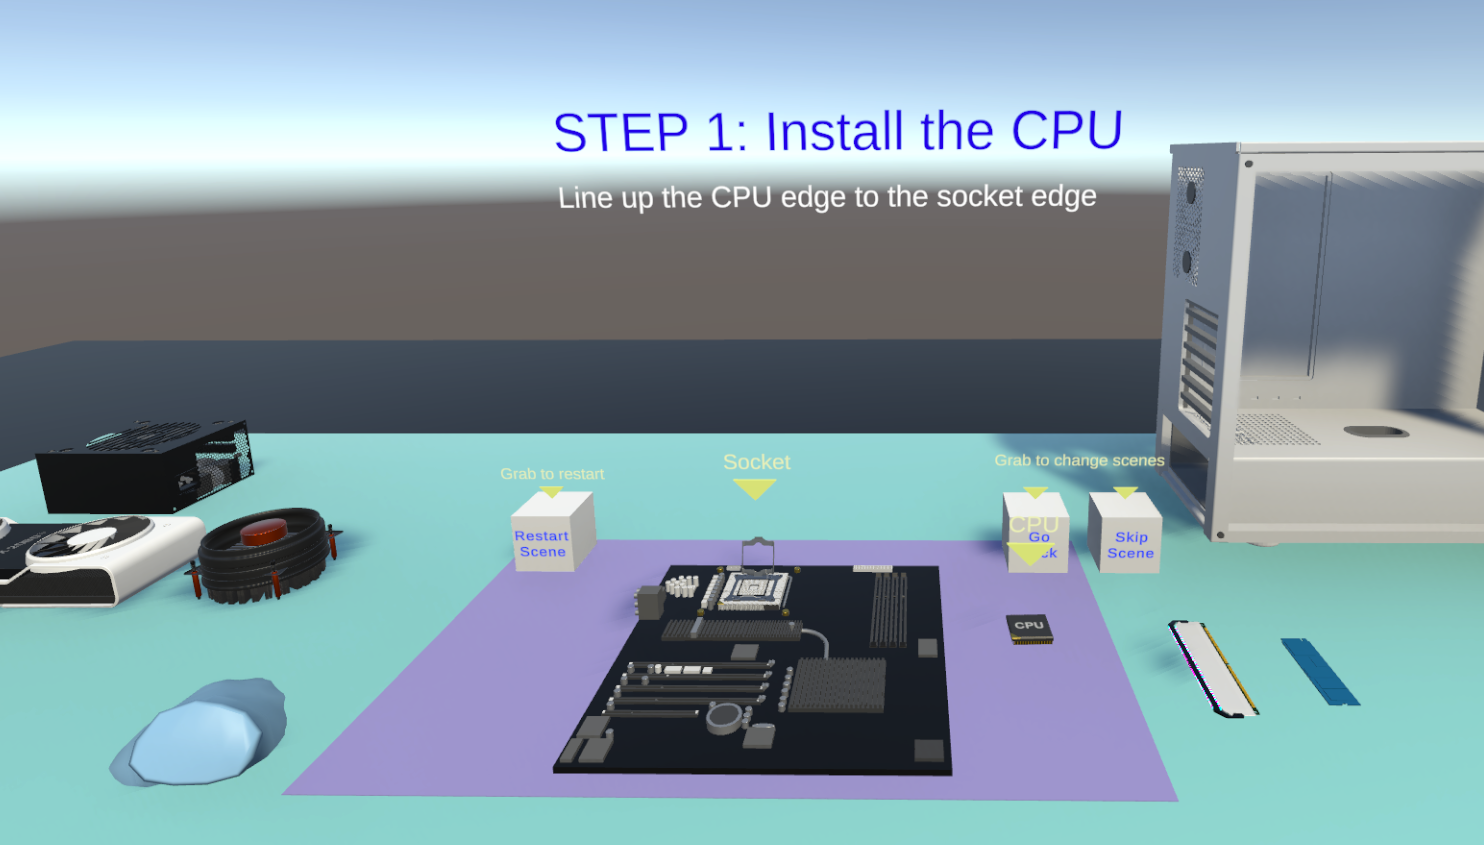
\includegraphics[width=5cm]{images/SetUp.png}
    \caption{The set up for the virtual environment.}
\end{figure}

\subsection{Installation Scenes}

\par Each hardware component will have an designated installation scene. During these scenes, the important components are the main focus and the unnecessary components are not be displayed. To focus on components, scale and object angles may be altered to provide a better visual experience for the user. For example, the smaller components are enlarged and angled to give users a better perspective during the installation [Figure 11]. This allows users to see the latches, levers, slots, and ports more clearly. These individual install scenes contribute to users achieving a clear understanding of the installation steps and skills required.  

\begin{figure}
    \centering
    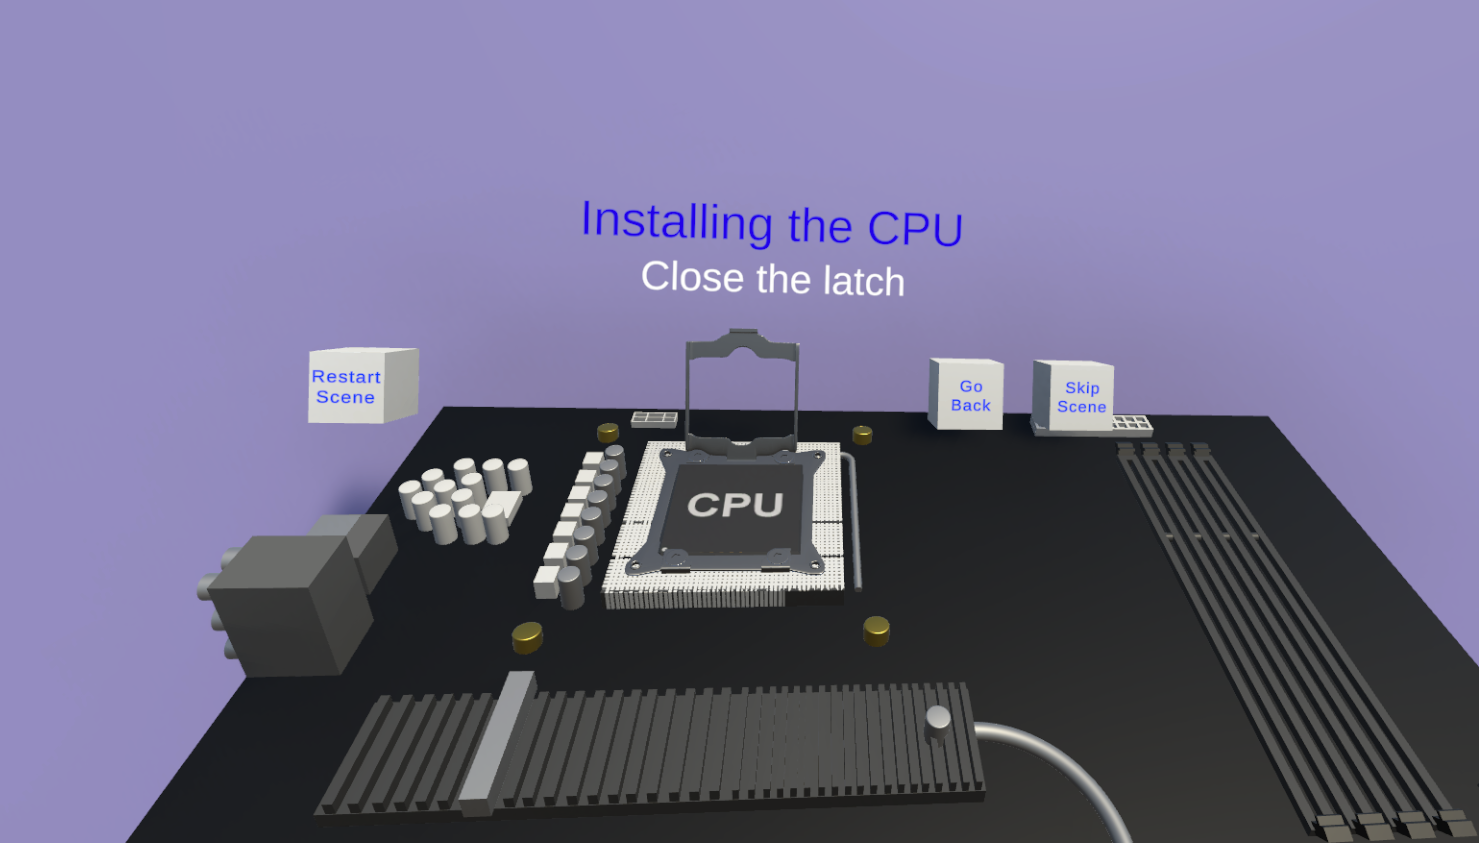
\includegraphics[width=5cm]{images/CPUInstallScene.png}
    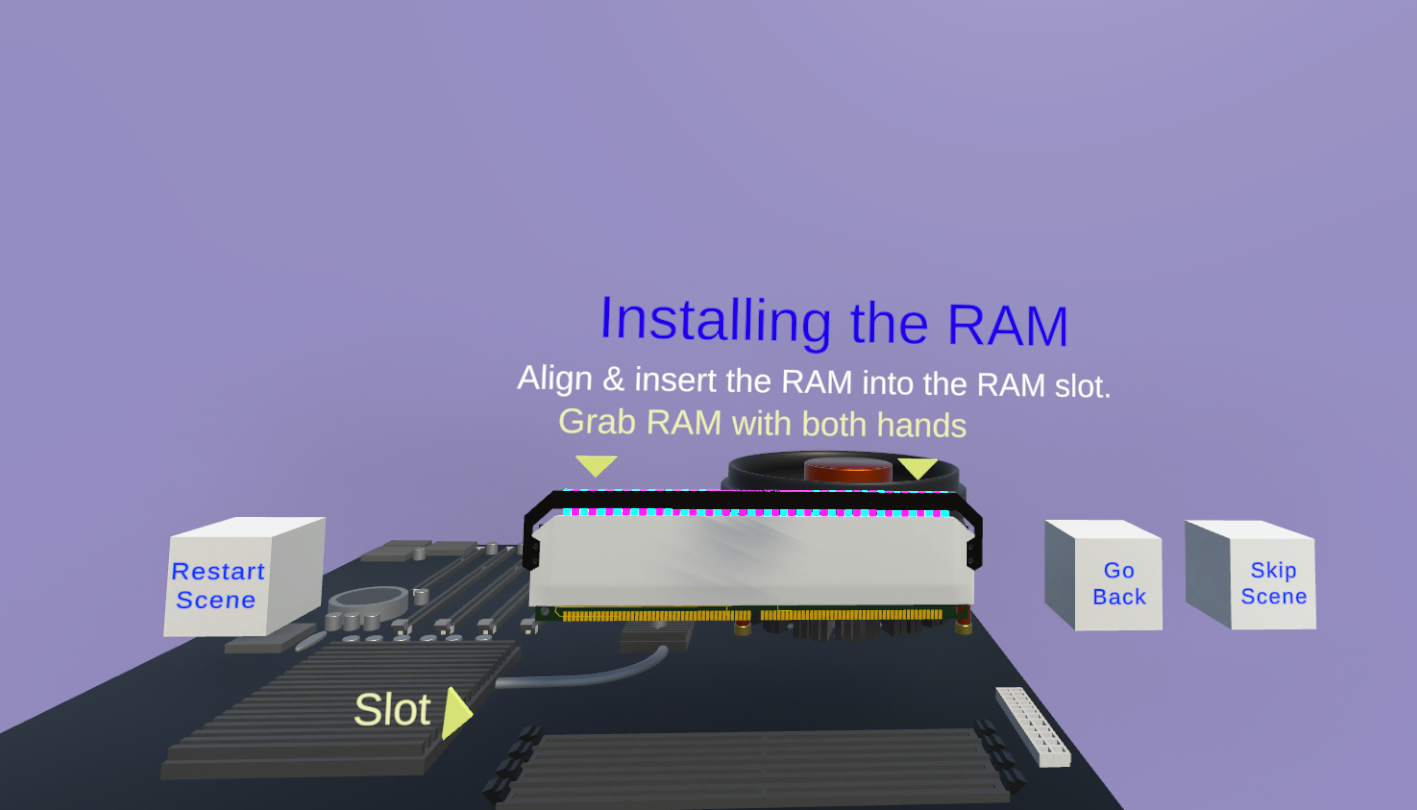
\includegraphics[width=5cm]{images/RAMInstallScene.png}
    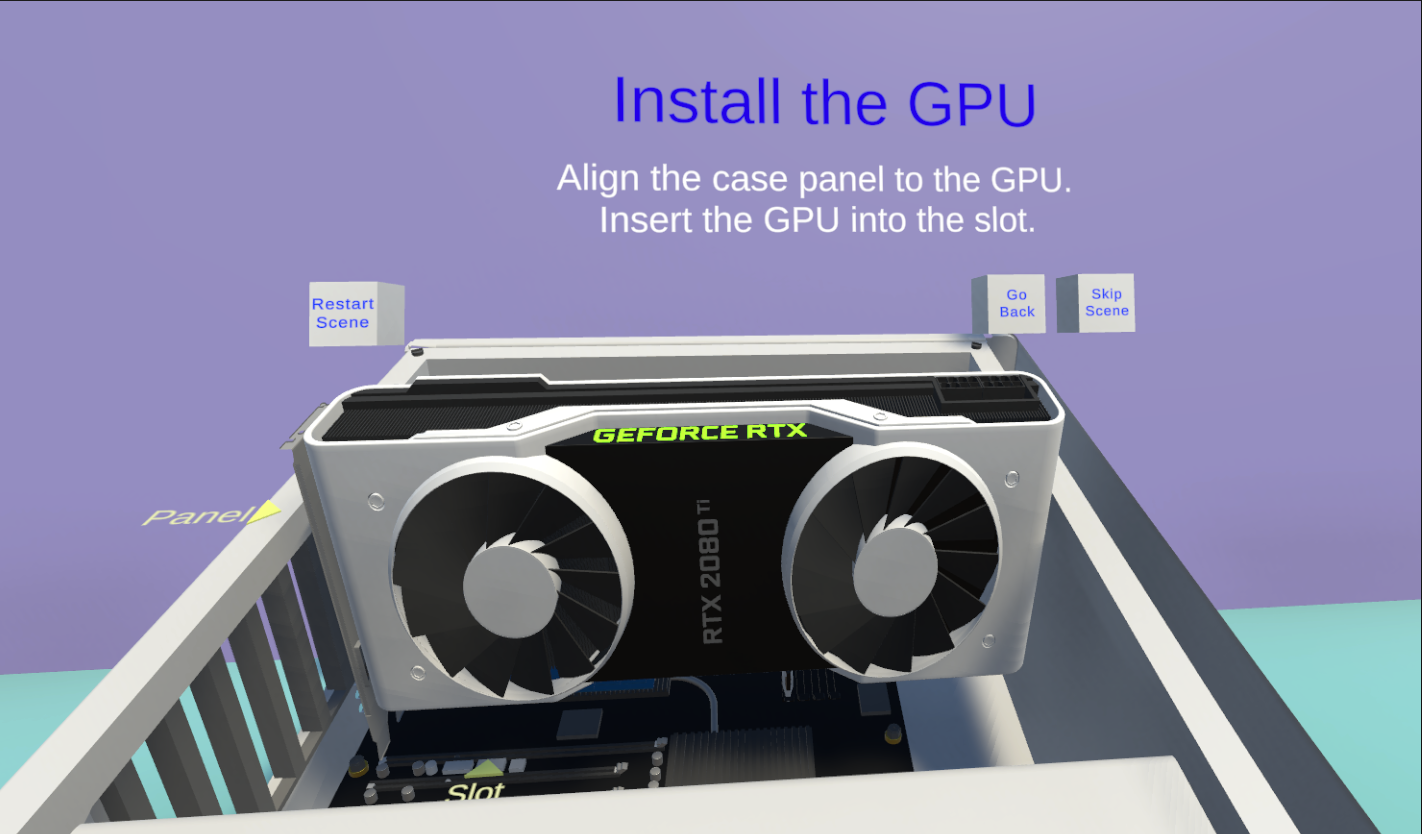
\includegraphics[width=5cm]{images/GPUInstallScene.png}
    \caption{The CPU, RAM, \& GPU install scene.}
\end{figure}

\par To avoid user discomfort, the ability to move around via the joysticks will be disabled for text-heavy scenes. Studies on VR show that the technology technology commonly contributes feelings of nausea, fatigue, dizziness, and bodily disorientation \cite{Spiegel2018TheEthicsOf}. Avoiding user movement during scenes with text helps prevent these feelings of dizziness or nausea in the virtual environment. Once the user completes the informational and motion instructional scenes, they will be able to move around in the environment using the controller joysticks. These user restrictions provide users with a more pleasant experience and help users focus on the informational aspects of the platform. 

\subsection{VR Interactions}

\par There are four main interactions that are used to install the components. These interactions include grabbing components, screwing in components, closing hinged components, and placing/connecting components. 

\subsubsection{Grabbing Components}

\par One of the most important interactions is the ability to grab components in the virtual environment. Users can grab objects by hovering the controller over it and pressing the Primary Hand Trigger on the controller \cite{Valem2022HowToVR}. Users are able to grab most objects, however to enhance the focus of particular components, the grab interaction may be disabled for some objects in certain scenes. The grabbing interaction also generates a custom ‘grab-hand’ pose when users grab an object [Figure 1]. This changes the hand joints rotation to simulate a realistic hand pose when users grab the object \cite{Valem2022GrabHand}. This makes the grab interaction more realistic and accurate to the real task. 

\subsubsection{Screwdriver Motion}

\par There are many approaches to simulate the screwing motion. One approach is to have users perform the rotating motion with the controller to trigger the objects the screwdriver collides with. This approach requires the detection of such movement using a custom script \cite{Valem2020HowToDetect}. Another approach is to have the screwdriver behavior begin when a trigger on the controller is pressed. This approach requires users to press an additional trigger on the controller since they would already be using the Primary Hand Trigger to grab the screwdriver. Instead, this project implements a much simpler approach. 

\begin{figure}
    \centering
    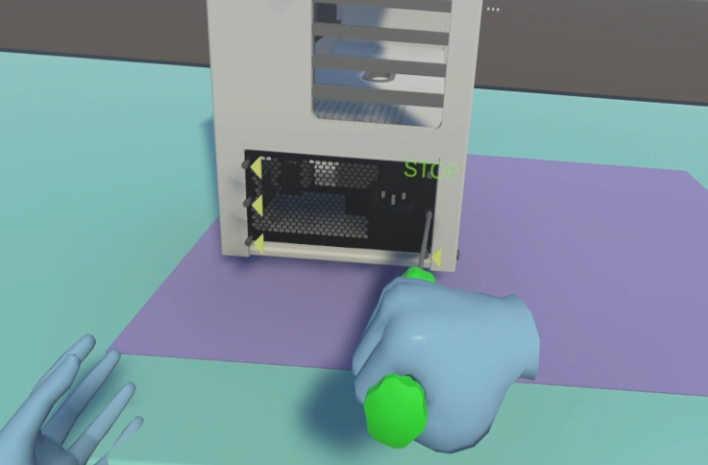
\includegraphics[width=7cm]{images/ScrewdriverUI2.png}
    \caption{UI text displays to let the user know the screwing interaction is complete.}
\end{figure}

\par To use the screwdriver, the user aligns the screwdriver tip over the screw to trigger the screwing behavior. The screwing animation will begin when the tip is colliding with the corresponding screw object, which will use a script to alter its position and simulate being screwed in \cite{Valem2022HowToVR}. For the installations that require the screwdriver interaction, there is additional user interface (UI) text that guides the user throughout the interaction. This UI text points out the screws that will trigger the screwing behavior. The UI text will also let the user know when the screws are tight enough [Figure 12]. The looseness of screws may be difficult to simulate in VR so the UI text helps simulate this factor so users know when to move on. 

\subsubsection{CPU Installation}

\par Unity’s hinge component is used for the CPU installation. Using this component, the CPU lever and latch use a hinging behavior that connects with the CPU socket \cite{Unity2023HingeJointComponent}. To install the CPU, the user grabs and closes the latch/lever as they would a hinged panel. For this interaction, closing the latch and lever requires a small range of motion using the controller. Users close the latch/lever by first grabbing the objects and then moving them towards their closing position [Figure 13] \cite{Valem2022HowToVR}. An issue with closing the CPU latch and lever is scalability. Since the CPU's size is comparatively small to the user's hand in the virtual environment, the hinge behavior responds to smaller hand movements. As a result, the users will use a smaller range of motion to close the latch and lever rather than using a larger and more intuitive motion to close the latch/lever. Although the movements to close the CPU are not as intuitive as a full range of motion for closing a latch, it still provides a similar physical motion to simulate the CPU installation. 

\begin{figure}
    \centering
    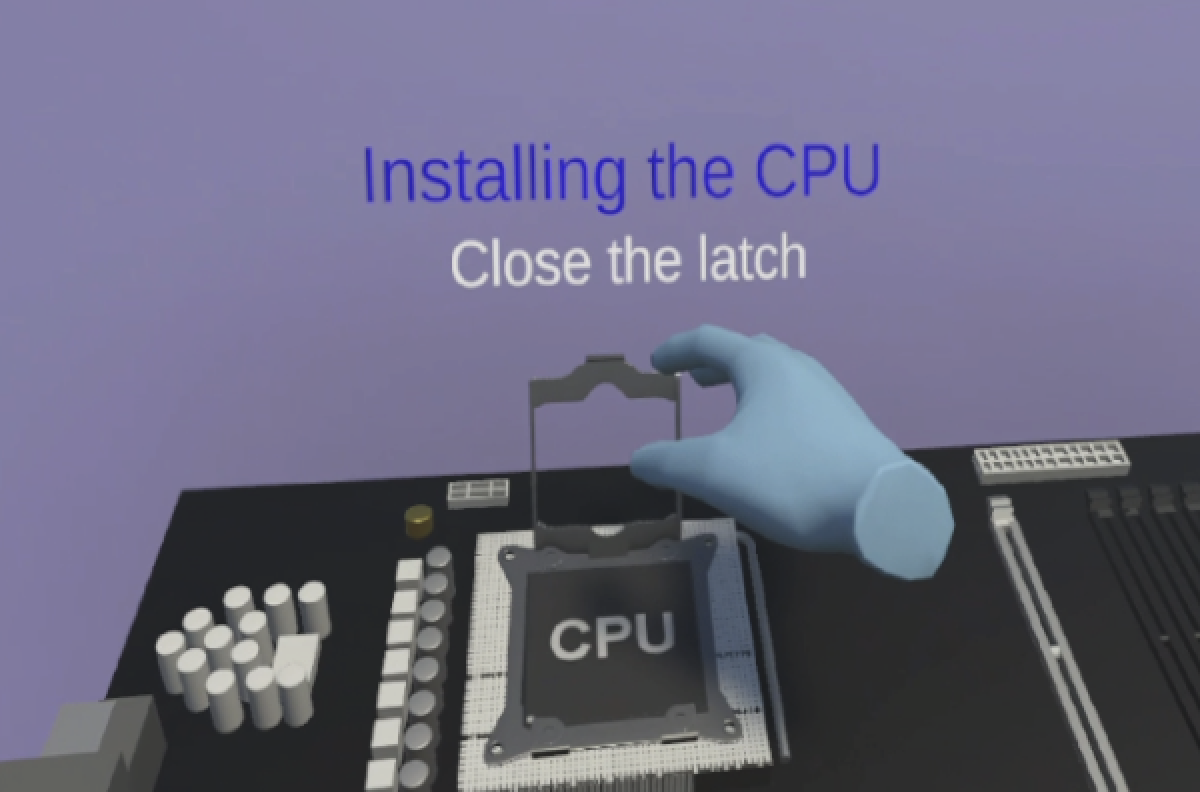
\includegraphics[width=7cm]{images/CPUHinge.png}
    \caption{The CPU has hinging behavior when the user interacts with it.}
\end{figure}

\subsubsection{Connecting \& Placing Components}

\par Another important interaction is connecting and placing hardware. This interaction is used in all the scenes where hardware is placed into their socket or wires are connected. For this interaction, the user must place the hardware near the port or socket area [Figure 14]. Then using drop zones, the hardware component will snap into place. The drop zones are Unity object components that allow for other objects to snap into place when they enter the drop zone \cite{Unity2023VRSnapZones}. To make the interaction more accurate, the drop zone can be minimized to ensure the user accurately aligns the component before it snaps into place. This interaction allows users to correctly install components as long as they are placed in the designated zone. 

\par The various sockets and ports also have defined objects they are able to interact with. This prevents the user from incorrectly installing components into the wrong socket. In other words, objects will not snap into place for an undesignated drop zone. The snap-in behavior provides additional guidance to users during installation since the hardware will snap into the installed position. This interaction is beneficial for newer users because it prevents incorrect installation. 

\begin{figure}
    \centering
    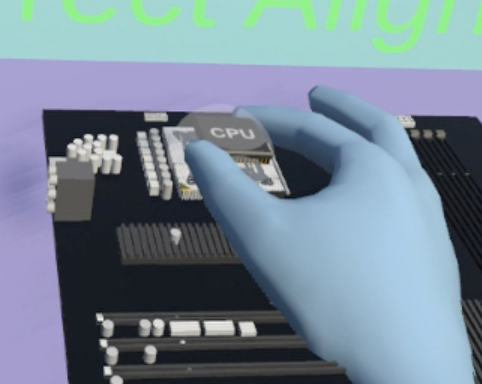
\includegraphics[width=7cm]{images/DropZone.png}
    \caption{The CPU snaps into place when the user drops it inside the drop zone.}
\end{figure}

\subsubsection{Developmental User Testing}

\par It is important to have accurate and intuitive interactions during the VR installations. User tests were conducted in order to ensure users responded positively to the main interactions. The first round of user tests focused on the motions for installing the CPU and the motions for screwing in hardware. These user tests also incorporated other basic interactions such as grabbing and placing objects. 

\par The goal of these user tests are to ensure that the user motions are not difficult and confusing to the user. These interactions should be intuitive in order to resemble the physical motions used in the real process. The test group includes novice and experienced users. Including different ranges of computer assembly knowledge provides useful feedback. The experienced users provide feedback helpful for platform accuracy and interaction intuitiveness. Whereas, novice users provide feedback helpful for the user experience and educational appeal.

\par The results showed that users had trouble understanding the motions they needed to perform during installation. Many users suggested including some sort of motion-related instructions to help with the interactions. Results also showed that users responded positively to simple interactions, such as the screwdriver interaction. Users found the screwdriver behavior very intuitive and easy to grasp since the screwing motion is triggered by simply aligning the screwdriver tip over the screw. 

\subsubsection{Motion-Related Instructions}

\par Based on the feedback from the initial round of user tests, motion-related scenes are included for each installation scene. In this scene, users are shown a preview of the installation process along with the motions needed to simulate it. This scene also includes brief text instructions regarding the installation process [Figure 15]. 

\begin{figure}
    \centering
    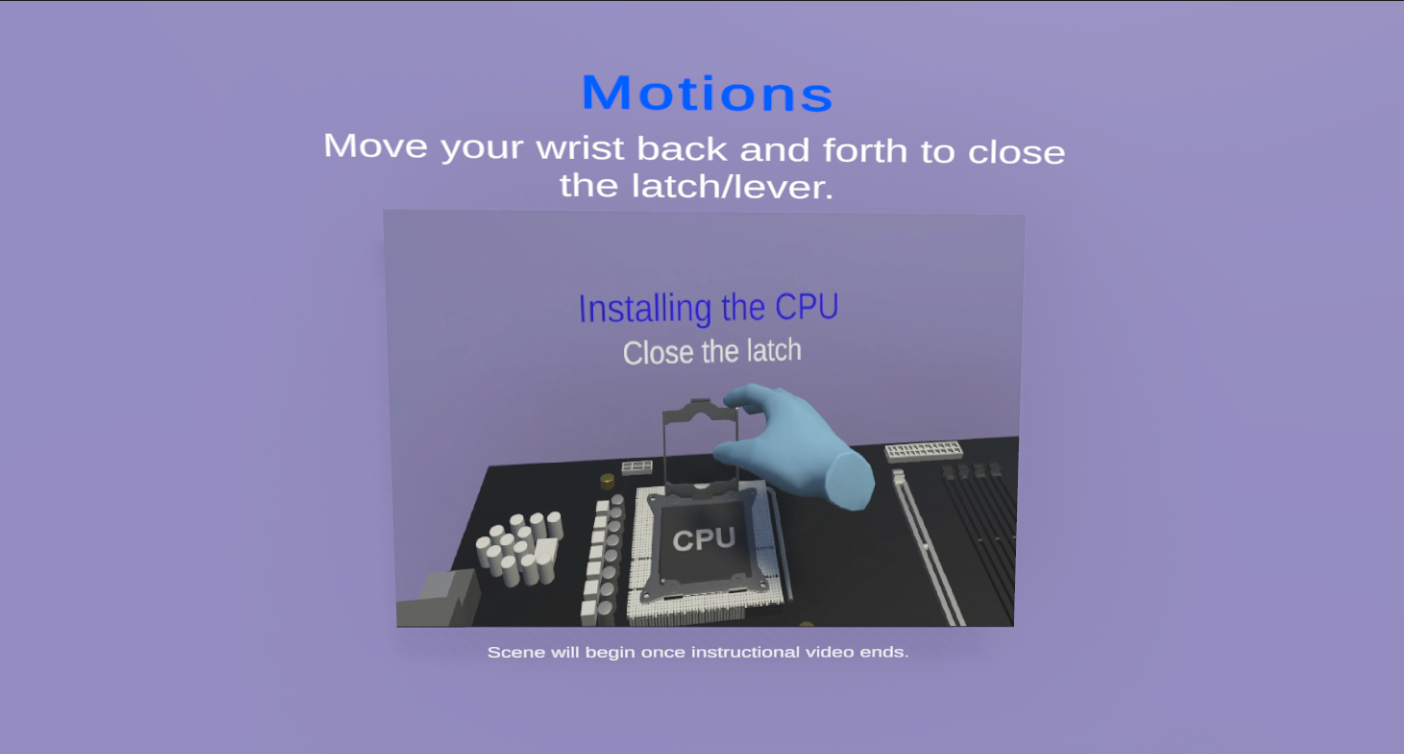
\includegraphics[width=7cm]{images/CPUmotions.png}
    \caption{The Motions scene shows users how to interact with objects during the installation.}
\end{figure}

\begin{figure}
    \centering
    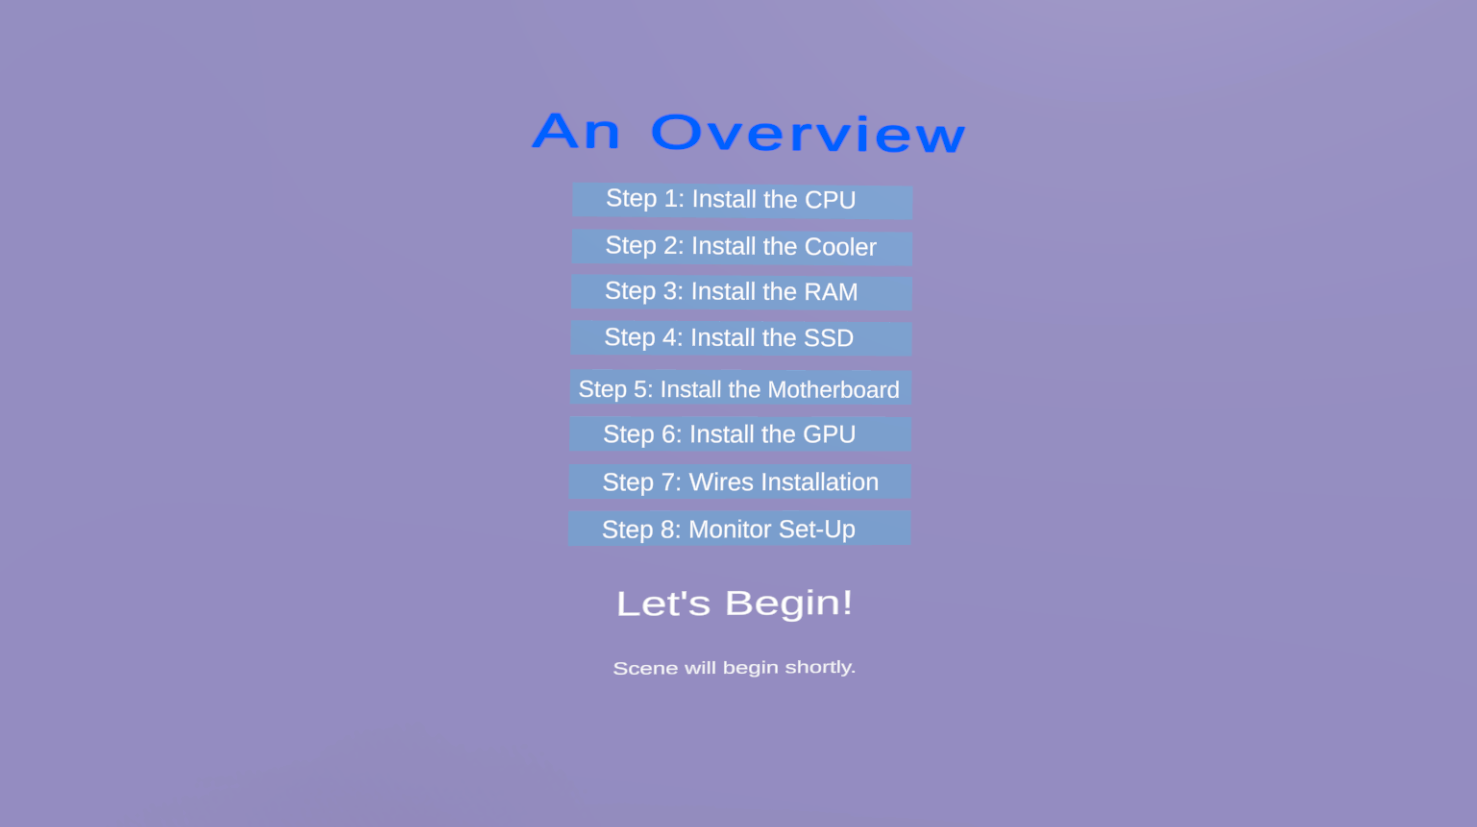
\includegraphics[width=7cm]{images/OverviewDiagram.png}
    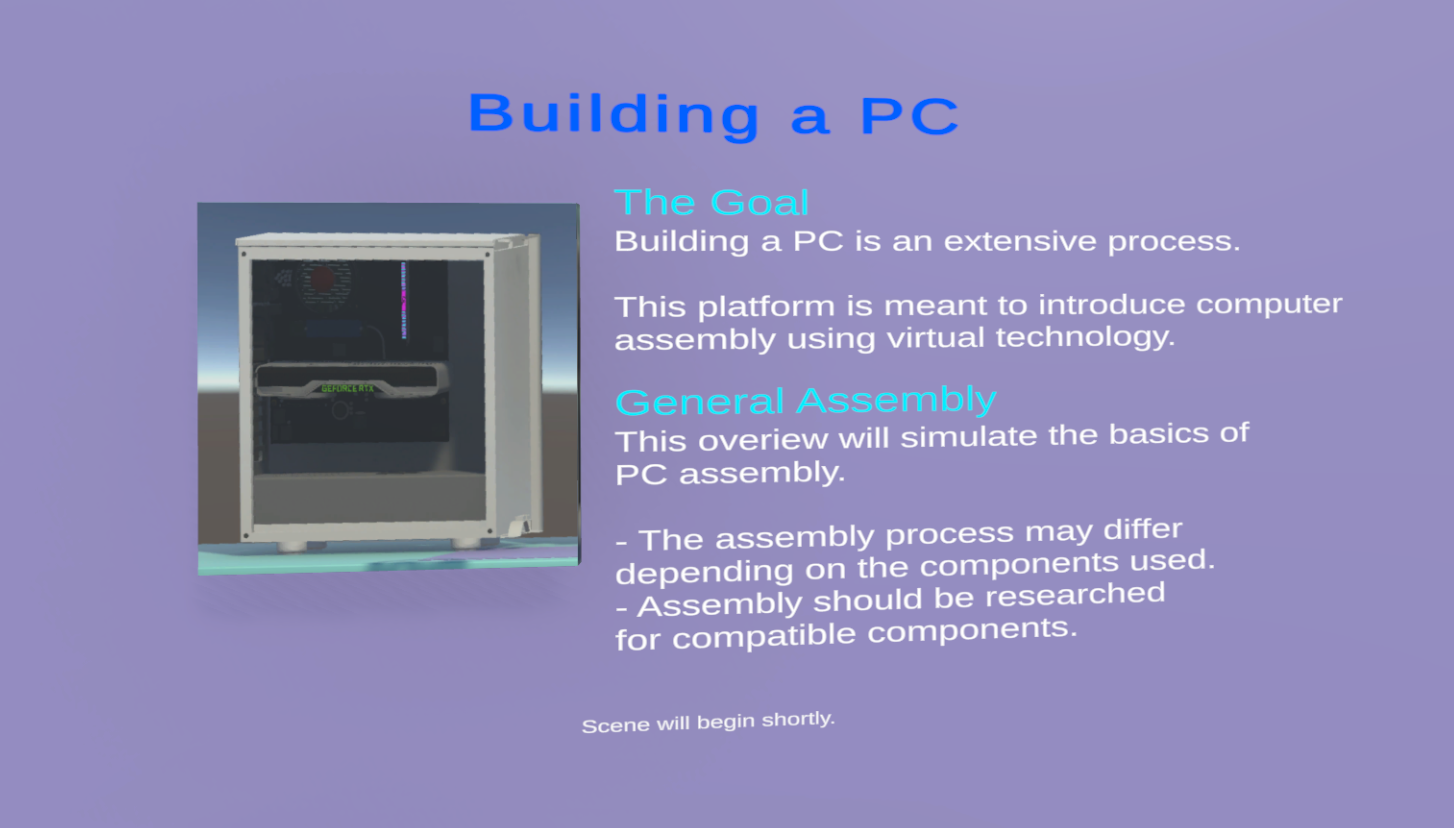
\includegraphics[width=7cm]{images/OverviewSummary.png}
    \caption{The summary and diagram of computer assembly in the VR platform.}
\end{figure}

\subsubsection{Educational Elements}

\par The platform incorporates various educational elements to help the user understand the installation process. These elements include an overview and diagram of the overall computer assembly process. This provides users an simple summary of the process before they begin to install the hardware. In particular, the diagram displays the installation steps in order. Including a summary and diagram of the process is meant to help users comprehension of computer assembly [Figure 16]. The goal is to effectively introduce the users to computer assembly.  

\par In consideration of the project’s target audience, the platform uses very simple instructions and definitions to explain each hardware installation. Any terminology that may be unfamiliar to the target audience is defined and installation steps are simplified. This is meant to avoid confusion for novice users.

\par To complete the installation process, users will connect the computer to a monitor, keyboard, and mouse [Figure 17]. This teaches users additional skills that may be necessary with the real computer assembly experience. It also provides users with a completed build that resembles a real computer setup. 

\begin{figure}
    \centering
    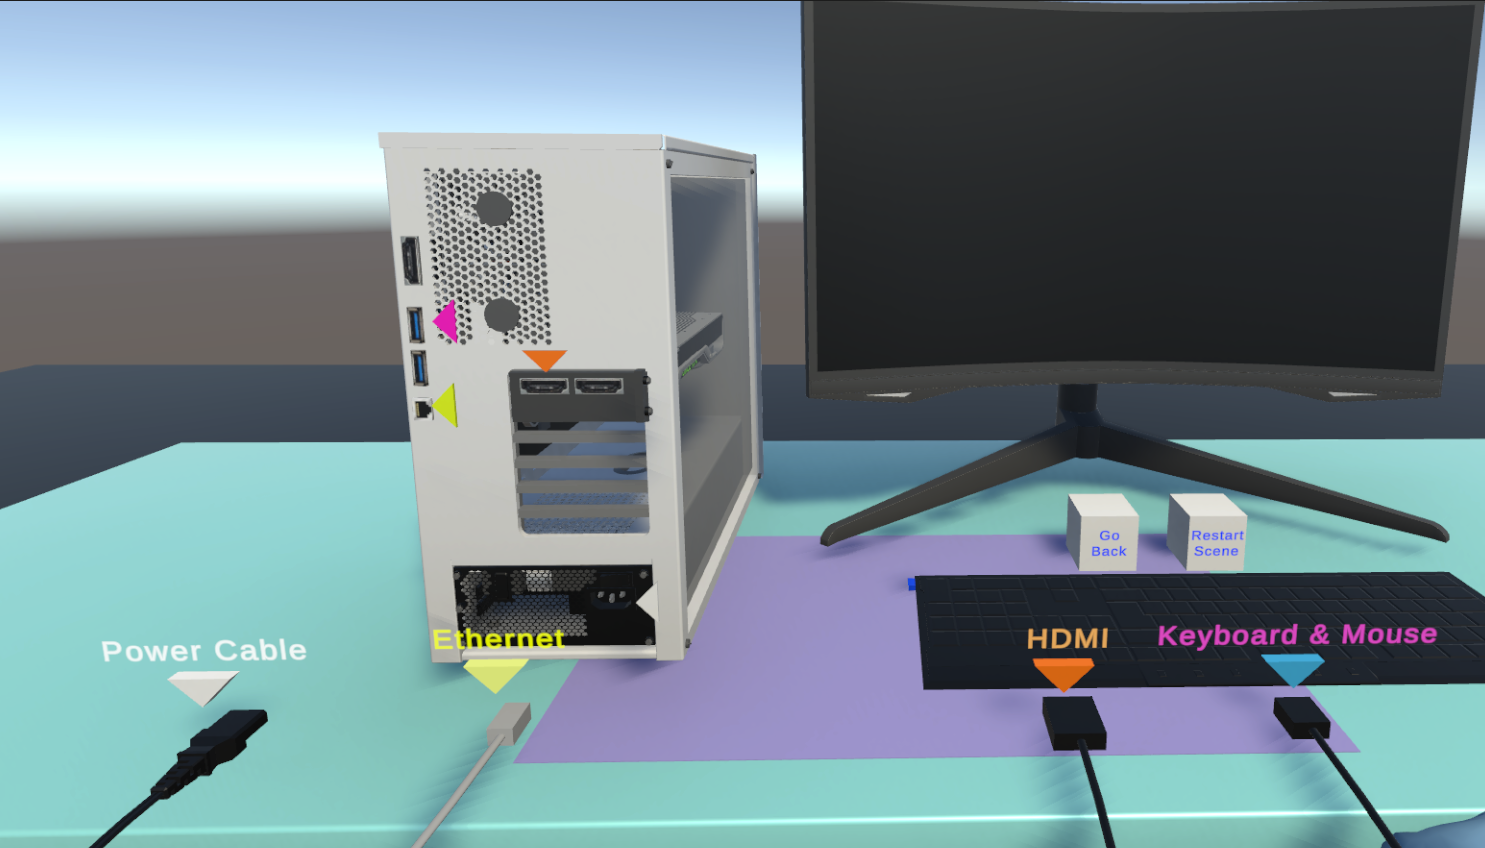
\includegraphics[width=7cm]{images/MonitorSetUp.png}
    \caption{The users will also simulate the monitor installation.}
\end{figure}

\subsubsection{Handling User errors}

\par In order to achieve the educational goals of the platform, it is important to consider user errors during the assembly process. To handle user errors, the platform displays a text warning the user if they align components incorrectly [Figure 18]. This emphasizes the importance of alignment for certain installation steps. 

\par The platform also incorporates options for restarting a scene, going to the previous scene, and skipping a scene ahead. To implement these options, the installation scenes are developed to be independent of each other. In other words, any errors made in previous scenes do not affect other scenes after. Each scene assumes all previous installation processes were completed correctly. This allows for users to make mistakes without the concern of affecting other installation scenes. It also gives users the freedom to move throughout the installation steps and repeat steps. In user testing, this option received positive feedback from users where they felt that it allowed them to repeat steps in the process and really understand the motions in VR. 

\begin{figure}
    \centering
    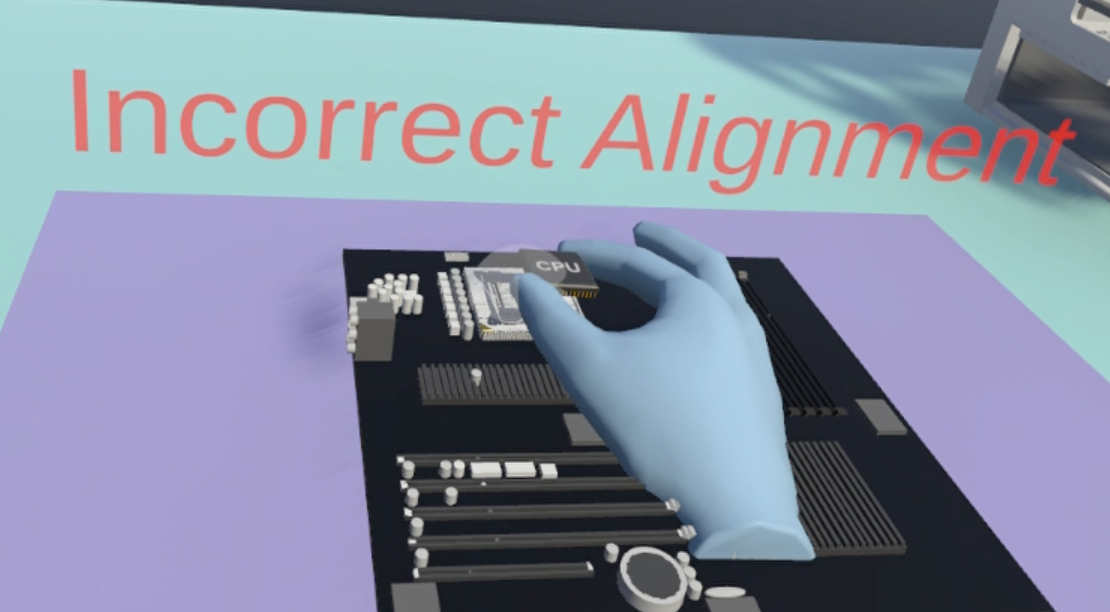
\includegraphics[width=7cm]{images/ErrorHandling.png}
    \caption{A UI text warns users of incorrect alignment during installation.}
\end{figure}

\begin{figure}
    \centering
    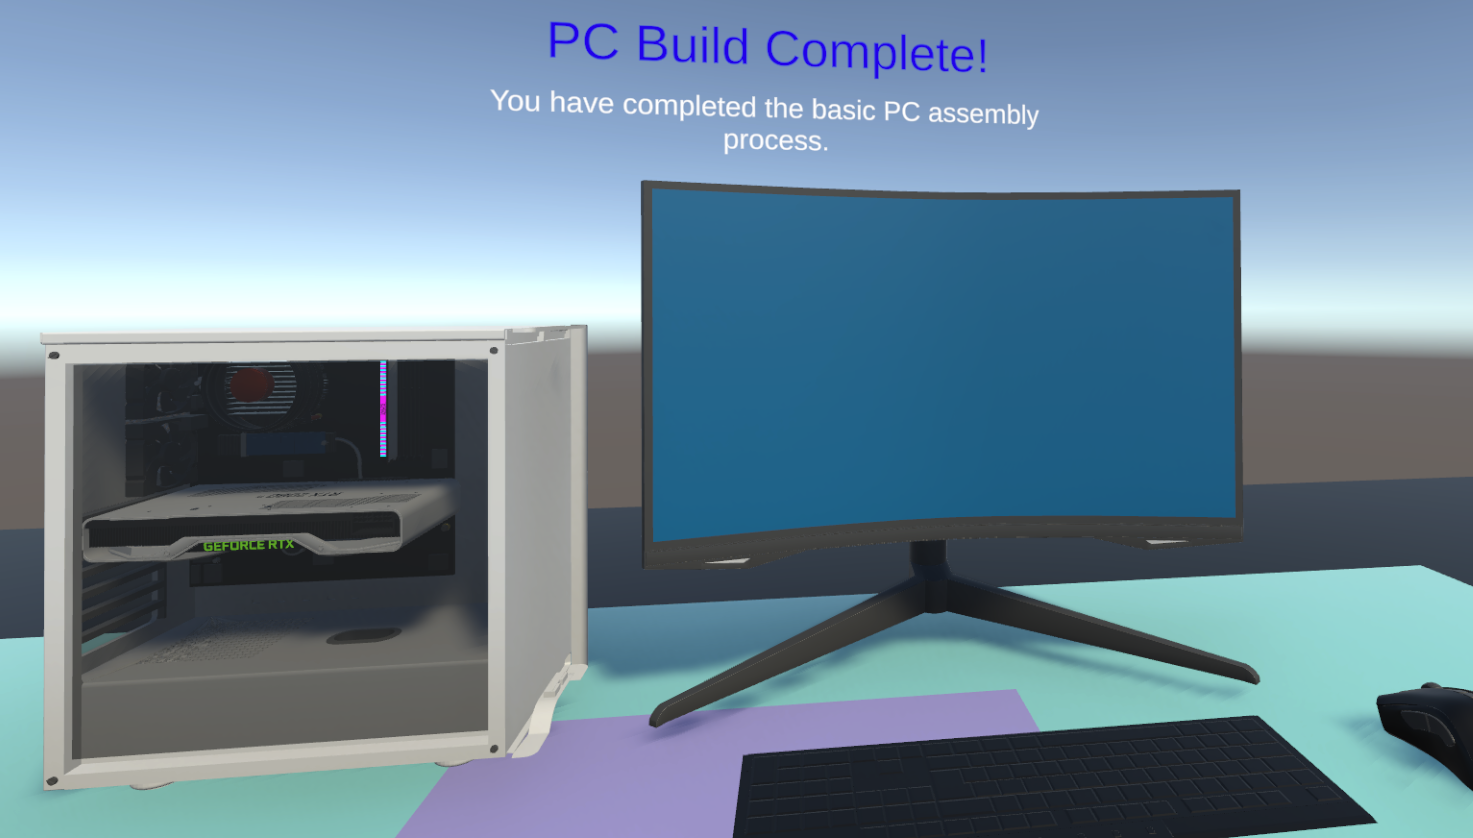
\includegraphics[width=7cm]{images/CompletedBuild.png}
    \caption{The completed PC and monitor set up.}
\end{figure}

\subsubsection{Final User Testing}

\par The final round of user testing consisted of novice and experienced users. The user tests consisted of users testing the platform and filling out a survey. The interview questions and responses are available in the final paper GitHub repository. This survey focused on the user experience and the educational outcomes of the platform. The purpose of the survey is to test whether users were satisfied with the VR experience and benefited from the educational goals of the platform. The platform was tested by 8 users, where 62.6\% were users who had experience in building a PC and 37.5\% were users who had never built a PC before. Including both groups in the user group helped tailor the platform for novice and experienced individuals. 

\begin{figure}
    \centering
    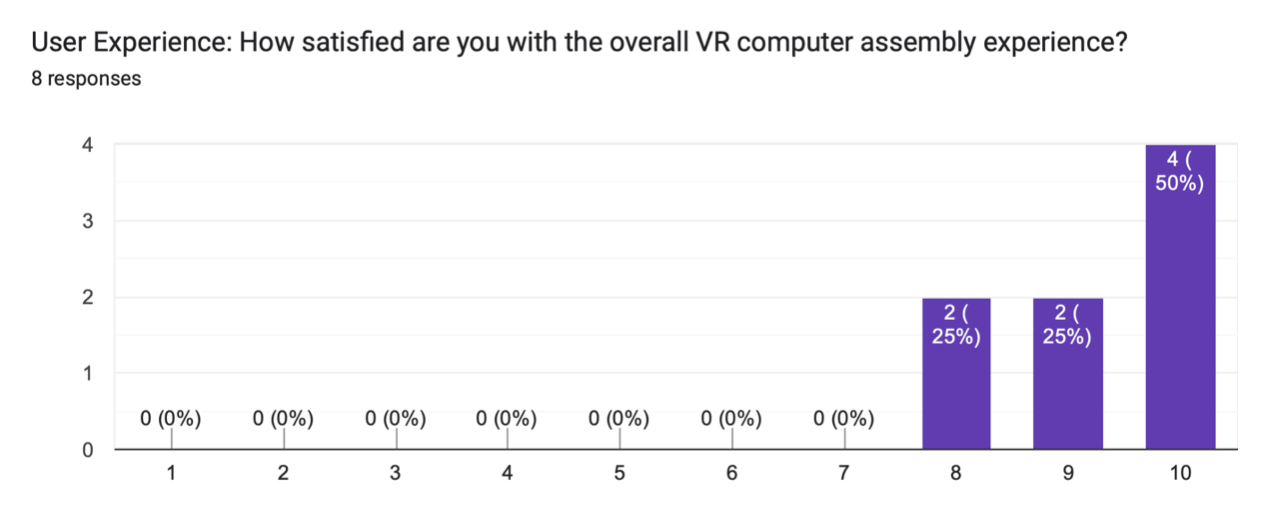
\includegraphics[width=9cm]{images/VRSatisfaction.png}
    \caption{The users satisfaction with the VR platform.}
\end{figure}

\par To evaluate the effectiveness of VR, users were asked whether they had used VR in the past. The feedback revealed that 62.5\% of users had used VR in the past. The feedback also showed that 100\% of users were satisfied with the VR experience [Figure 20]. More importantly, more than 50\% of users agreed that the platform was easy to navigate and interact with and 87.5\% of users were highly satisfied with the responsiveness and smoothness of the platform.  

\par Users were also asked about their computer assembly knowledge prior to using the platform. The users had different levels of computer assembly knowledge. 20\% of users had very little computer assembly knowledge and 50\% of users had a higher level of computer assembly knowledge [Figure 21]. The results revealed that 87.5\% of users felt that they had better knowledge of the computer assembly process. More specifically, experienced users mentioned that the platform reinforced previous knowledge of computer assembly and novice users felt that the platform introduced the basic assembly process. More than 50\% of users felt relatively high levels of confidence in researching/preparing for the computer assembly process after using the platform [Figure 22].

\par The surveys also allowed users to make suggestions and comments about their experience. Some users suggested having more freedom to skip instructional scenes. This would benefit users with more experience who may not need to read the information or motion instructions. Some users also suggested including a list of tools required during assembly. They felt that it would add to the educational aspect of the platform. More experienced users also pointed out a missing installation step in the platform, where the platform skipped the GPU wire installation. 

\begin{figure}
    \centering
    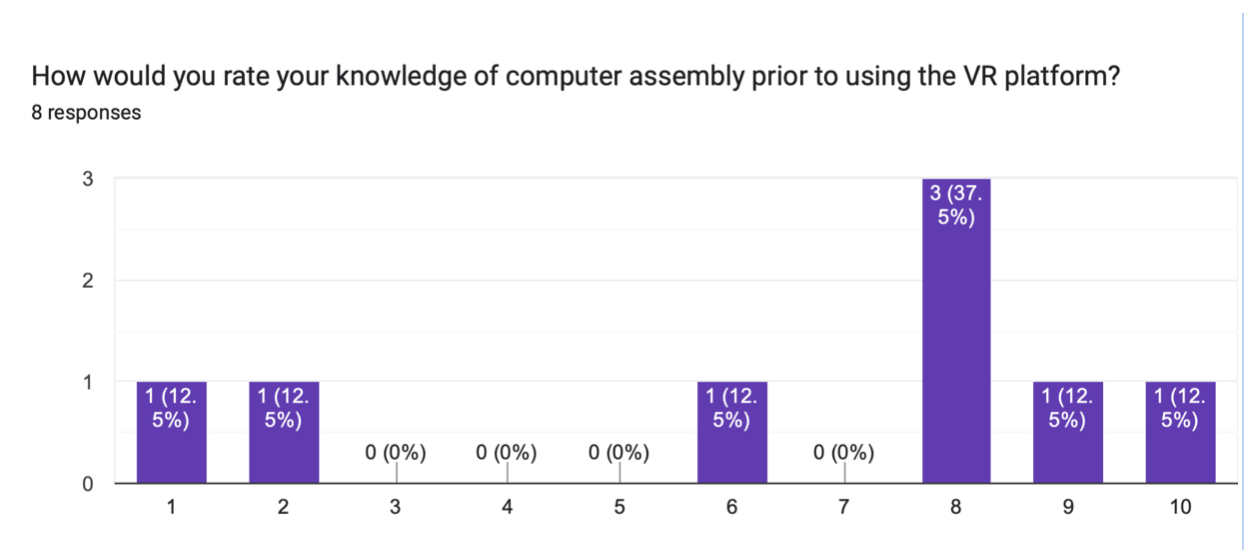
\includegraphics[width=9cm]{images/PriorVRKnowledge.png}
    \caption{The users responses prior to using the VR platform.}
\end{figure}

\begin{figure}
    \centering
    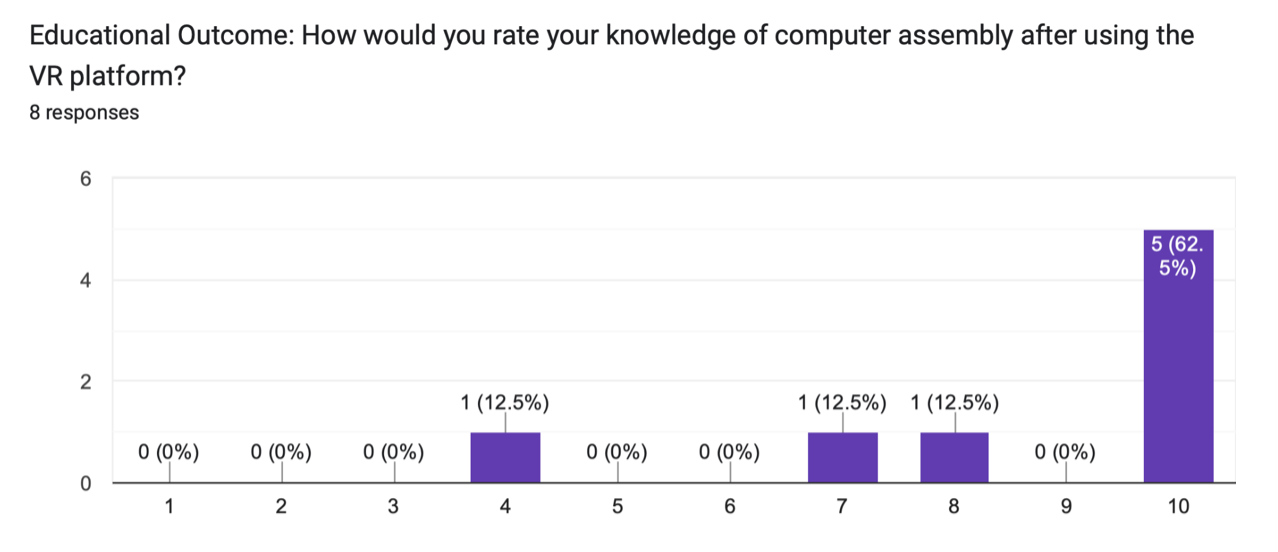
\includegraphics[width=9cm]{images/UserExperience4.png}
    \caption{The users responses after using the VR platform.}
\end{figure}

\par Most importantly, all the users agreed in recommending the platform as a resource for learning/preparing for computer assembly. However, experienced users emphasized that this platform was not meant to replace preparation and research for computer assembly. 

\section{Evaluation Metrics}

\par The evaluation metrics for this project measure the effectiveness of virtual reality and the educational aspects of the platform. 

\subsubsection{Virtual Reality Metrics}

\par Virtual reality has the capability to enrich many experiences in gaming, entertainment, education, etc. There are studies that observe the elements of VR which contribute to a successful experience. Research on effective VR introduces the VR PLAY guidelines created to assist in evaluating and designing an effective VR user experience \cite{Desurvire2018DesignUserExperience}. The study provides metrics of success for VR platforms based on research conducted using extensive experience with player research and further discussion on VR research. 
This results determined the relationship between presence, embodiment, ethics, and physicality with the success of a VR game. To determine the effectiveness of these five elements in VR, the study analyzed five categories: Usability, Playability, VR Immersion, Creative VR, and New Player Experience \cite{Desurvire2018DesignUserExperience}. 

\par In conclusion, the heuristics used to develop the VR PLAY guidelines demonstrated accuracy in measuring VR success. For this project, we will focus on using presence, embodiment, and physicality to measure the VR experience. 

\begin{itemize}
    \item \textbf{Presence:} This metric measures the level of the user's physical presence in the virtual environment. This is the key element in VR immersion, since VR creates an illusion of a “real” world. Creating a sense of presence is vital for a VR platform.
    \item \textbf{Embodiment:} Very similar to presence, embodiment measures the extent to which the player in the VR environment identifies with the body of the player character. This embodiment contributes to user engagement and decision-making in the virtual world. In other words, measuring embodiment also measures some level of player enjoyment. 
    \item \textbf{Physicality:} This metric considers the player's physical comfort, ability to perform the actions of the game, and need for breaks or cool-down time between periods of intense physical activity. This also considers the player's tendency to develop feelings of dizziness, nausea, etc. when in the virtual environment. 
\end{itemize}

\par There are various other evaluation metrics that measure different elements of VR games. For instance, VR games can be evaluated based on user satisfaction of the gamification elements in the platform. These metrics tend to focus on the content and entertainment factors of a platform rather than the physical and functional elements of VR \cite{Desurvire2018DesignUserExperience}. 

\par On the other hand, the heuristics behind the VR PLAY guidelines demonstrate more solid foundations for ensuring success in a virtual reality experience. These categories focus on measuring the elements of VR that make it unique to other mediums. Due to this project’s emphasis on user interaction in the virtual world, the metrics behind the VR PLAY guidelines measure more relevant factors to our project's goals. Our use of VR is highly attributed to its ability to increase user engagement, thus making presence, embodiment, and physicality ideal metrics to consider. 

\section{Educational Metrics}

\par This project targets users unfamiliar with computer assembly, however experienced users are also considered. The educational goal of the platform is to introduce users to the overall process and skills necessary to assemble a computer. To evaluate th educational goals, the educational metrics measure the users' knowledge of computer assembly after using the platform. The level of users' confidence in computer assembly after using the platform also help determine whether the project achieved its educational goals. The main educational criteria is the following: 

\begin{itemize}
    \item The platform strengthened user knowledge of computer assembly to some degree. 
    \item The platform served as a helpful preparation resource for the computer assembly experience .
    \item Users learned the overall computer assembly process.
\end{itemize}

\par To assess the educational success of this project, user testing is conducted along with a post-survey assessing user experience and educational outcomes. A similar study conducted user testing on an educational VR platform using surveys \cite{Chen2011AVirtualRealityExperiment}. The study evaluated the learning effectiveness of their platform by collecting data using questionnaires before and after user testing. Using the questionnaire feedback, the study concluded that their VR program was effective at increasing the students’ understanding of computer hardware in the course. For this project, the feedback from users will be collected using a similar method. The data will then be measured against the educational evaluation metrics.

\section{Results and Discussion}

\par The final survey results were compared with the VR evaluation metrics and educational evaluation metrics. In order for the platform to have achieved its goals, it must succeed as a VR experience and as an educational resource. 

\subsection{Presence}

\par The platform incorporates a 3D virtual environment in which the user can interact and move around in. Although some scenes have restrictions on movement, the interaction scenes allow free movement and interaction with objects in the virtual environment. Some limitations to presence in our platform include limited movement in informational and instructional scenes. Nonetheless, the final user tests show that the entire user group was satisfied with the virtual environment. This suggests that the platform successfully considered presence for the user in the 3D environment. 

\subsection{Embodiment}

\par The platform allows users to engage with virtual objects using the controllers. In the environment, these controllers are the hands of the players, thus contributing to user identification with the body of the player. Some limits to embodiment include no other physical body to the player. Users only have hand models to interact with other objects in the scene. To measure embodiment in the surveys, users were asked to rate the navigation and interaction as a player using their virtual body. The results showed that more than half of the users found the platform navigable and interactable. Thus, the platform achieved sufficient embodiment for the users to complete the PC build. 

\subsection{Physicality}

\par To achieve some level of physicality, the platform first considers the users’ pace throughout the game. This is done using the instructional and informational scenes, where users limit their interactions with the virtual objects in the environment. This provides some scenes for users to 'cool down' and rest from VR interactions \cite{Desurvire2018DesignUserExperience}. Next the platform considers user comfort. To do this,the platform avoids VR design that may increase feeling of nausea or dizziness in users. For scenes that are text-heavy, the platform avoids heavy user movement. This is meant to reduce discomfort for the user. The surveys show that most users were highly satisfied with the smoothness of the platform and did not mention any particular discomforts. 

\par Finally, user feedback suggests that the platform adequately achieves its educational goals in serving as a resource for introducing computer assembly. According to the responses, more than half of users felt more confident in their computer assembly knowledge after using the platform. More experienced users felt that the platform served as a reinforcement of their current computer assembly knowledge. Whereas novice users felt that the platform was helpful in introducing the process for this first time. In the end, the user feedback demonstrates that the platform sufficiently achieved its educational goals for novice users. However, for more experienced users, the platform does not strengthen their current knowledge, but reaffirms it. These users also mentioned that they would recommend the platform to others as a preparation resource, with the caveat that the platform does not replace the complete computer assembly preparation process. 

\subsection{Future Work}

\par Although the evaluation metrics reveal that the platform provides a successful VR experience and achieves its education goals, there are many aspects of the platform that can be improved. Suggestions from the user surveys include improving the user interface to make the platform more enjoyable for experienced users. This includes adding options to skip informational scenes and including more elements considering compatibility of hardware. To consider compatibility would also increase the level of computer assembly that the platform teaches. If the platform were to introduce the concept of compatibility to novice users, it must include the educational elements  and VR interactions to accurately portray compatibility in VR. 

\section{Ethical Considerations}

\subsection{Cybersickness}

\par There are general ethical concerns surrounding virtual technology. Studies of VR technology reveal that reality technologies may contribute to physical, mental, and behavioral harms. These issues are important to consider when developing a platform hosted using virtual technology. 

\par VR technology raises moral concerns regarding the physical and mental health of users since it may pose harms related to "Cybersickness"\footnote{a term that has been coined to describe the feelings of nausea, fatigue, dizziness, and bodily disorientation that users frequently experience following a VR session.}, PTSD\footnote{Post-Traumatic Stress Disorder}, and bodily neglect. Users may also experience prolonged difficulty adjusting to the real world \cite{Spiegel2018TheEthicsOf}. Moreover, VR’s increasing ability to stimulate the range of senses beyond sight and sound also increases the chances of users experiencing similar triggers to that seen in PTSD \cite{Kenwright2018VirtualRealityEthical}. 
Users of virtual technologies may also experience personal or bodily neglect. Risks include possible illness and fatalities due to users neglecting their own physical well-being \cite{Spiegel2018TheEthicsOf}. As VR technology continues to grow, the reports of extreme self neglect are likely to increase as well. Consequently, VR not only poses a potential harm to users' mental health, but also to their physical wellness. 
	
\par To address this ethical concern, this project aims to reduce the feelings of nausea, fatigue, dizziness, and bodily disorientation that are attributed with Cybersickness. This is done by applying VR design techniques that reduce the likelihood of the harmful effects. An example is avoiding simultaneous reading and movement in the virtual environment. The virtual environment also takes a relatively short amount of time to walk the users through the entire computer assembly process. Due to the nature of this project, we focus on preventing the issue of Cybersickness and ignore PTSD and bodily neglect issues.   

\subsection{Education}

\par Over the years, there has been more incorporation of VR technology in education. The overlap between VR as a learning platform and education leads to VR ethical issues impacting individuals in education. The growth in technology has led to the introduction of reality technologies in classrooms to promote visual and engaged learning \cite{Pirker2020VRinCS}. Thus, general ethical concerns about virtual technology may impact students and pose a potential harm to their physical/mental health and their personal data. Although this project can potentially serve as a resource in education, it does not directly address the potential harmful effects of VR in education.

\subsection{Cost}

\par Building a personal computer is a constructive and expensive experience. Since many individuals can not access or afford to build their own PC, the VR PC Builder provides an accessible and more affordable alternative PC building experience. The overall cost of all the necessary hardware required to build a PC may be comparatively high to VR technology, however, reality technology is still expensive. Virtual learning environments are growing as a technology, yet commercial VR systems that offer sophisticated, complex, and diverse functions are expensive relative to personal computers \cite{Bricken1991VirtualRealityLearning}. As a result, the cost gap between personal computers and VR technology continues to be an issue of accessibility for the PC Builder. Although computer hardware ranges from hundreds to thousands of dollars, VR technology is still expensive and its cost ranges in the hundreds of dollars \cite{Alsop2023VRHeadsetAvg}. Thus, the cost of VR technology poses issues about accessibility and affordability.

\par Although this project does not consider this issue directly, there are potential solutions for accessing VR through institutions as a resource. As VR technologies grow, institutions provide the option to use VR as a resource. However, this platform does not solve the greater issue between technology accessibility and socioeconomic status.

\printbibliography

\appendix

\section{Replication Instructions}
\subsection{Installing Unity}

\begin{enumerate}
    \item Download the Unity Hub for your OS: \\https://unity.com/download.
    \item Select the latest version of Unity. This project uses version 2022.3.8f1.
\end{enumerate}

\begin{center}
    
\includegraphics[width=3cm]{replication images/Version.png}
\end{center}

\subsection{Installing Blender}

The Unity project uses blender 3D models for the hardware components. Install Blender before cloning the github repository. 

\begin{enumerate}
    \item Download Blender for your OS: 
    \\https://www.blender.org/download/
\end{enumerate}

\subsection{Clone GitHub repository}
\begin{enumerate}
    \item Open the terminal and navigate to a folder where you want to store the source code of the project. For this example, we will store the project on the desktop. 
        
    \begin{center}
        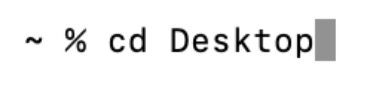
\includegraphics[width=5cm]{replication images/cdDesktop.png}
    \end{center}

    \item Now, use the clone command to clone the git repository. This may take a few minutes.

    \begin{center}
        
\includegraphics[width=10cm]{replication images/CloneCommand.png}
    \end{center}
    
\end{enumerate}
                       
\subsection{Opening the Repository on Unity} 
\begin{enumerate}
    \item Open the Unity Hub to see the projects menu. 

    \begin{center}
        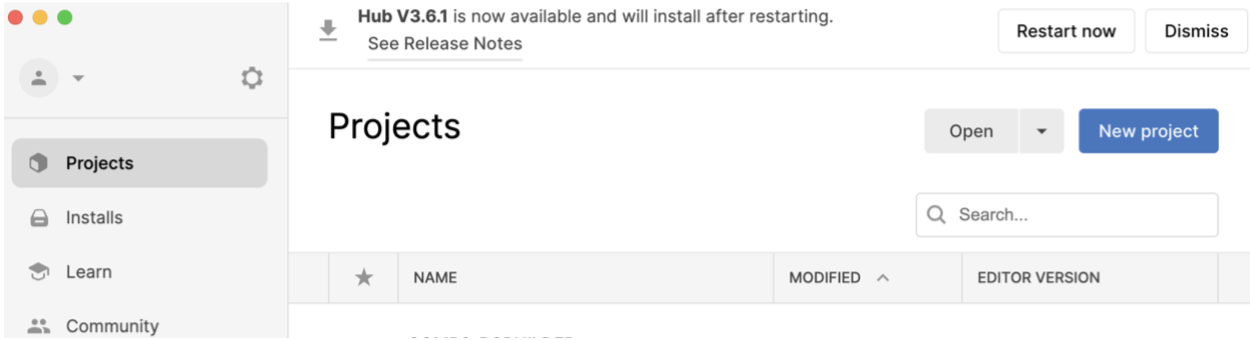
\includegraphics[width=9cm]{replication images/ProjectWindow.png}
    \end{center}

    \item Select the options to ‘Open’ a project and select ‘Add project from disk’.

    \begin{center}
        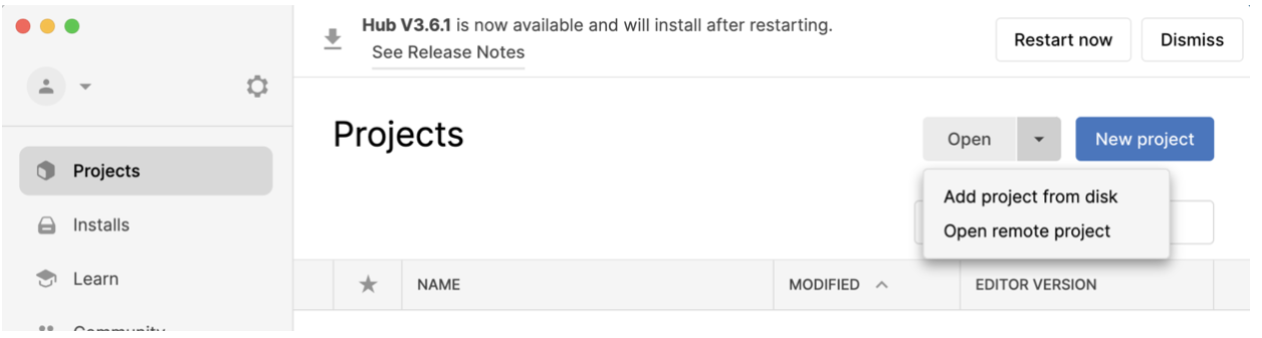
\includegraphics[width=9cm]{replication images/AddProject.png}
    \end{center}

    \item Select the cloned repository saved on your computer. 

    \begin{center}
        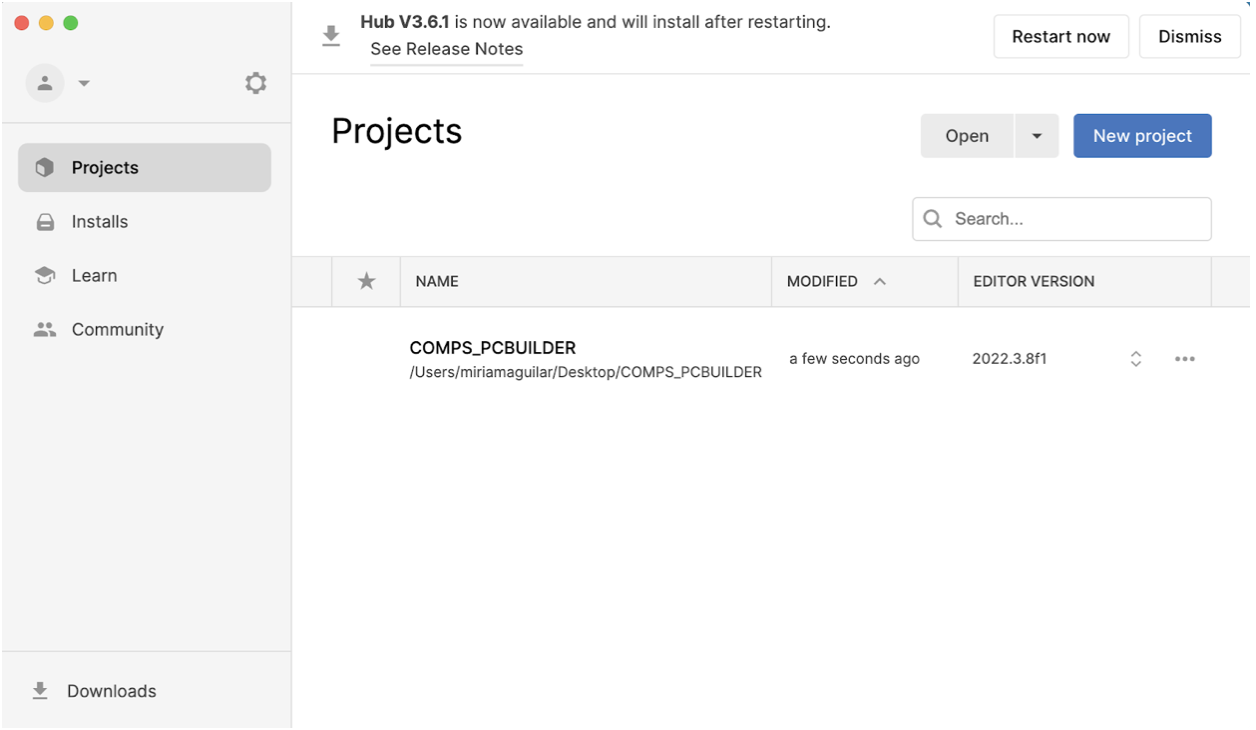
\includegraphics[width=8cm]{replication images/ProjectAdded.png}
    \end{center}

    \item Once the project is added to your projects, select it to open the Unity project. 
    
\end{enumerate}

\subsection{Downloading the Case 3D Model}

\begin{enumerate}
    \item The case.blend file is too large to upload to the git repository. In order to download the case model, download the blender file using this Google drive link: \\ \url{https://drive.google.com/file/d/1zDV5-eAq34c7GT_4SFE90QDLbL3oOGqE/view?usp=sharing}.
    
    \item Add the case.blend file to the \textbf{Assets/3D Models}
    folder. This is done by dragging the case.blend file from the desktop to the 3D Models folder.

    \begin{center}
        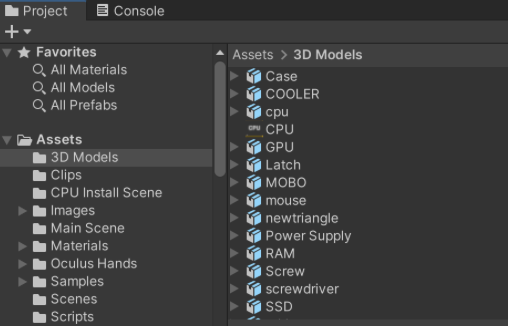
\includegraphics[width=7cm]{replication images/3DModels.png}
    \end{center}

    \item Manually add the case prefab to all the scenes with the missing Case Interactable. Drag the Case prefab from the 3D Model folder to the Prefab in the Inspector. 

     \begin{center}
        
\includegraphics[width=8cm]{replication images/AddedCaseModdel.png}
        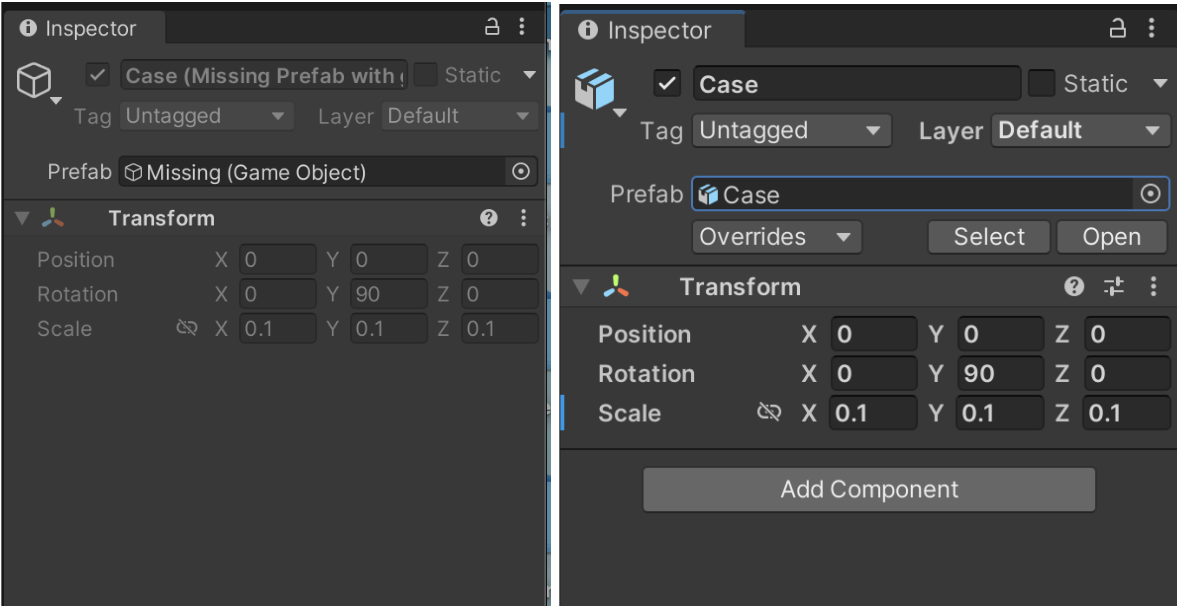
\includegraphics[width=8cm]{replication images/Inspector.png}
     \end{center}

    \item The platform should be ready to use. To view the scenes, go to \textbf{File {$>$} Build Settings}.

    \item The first scene of the platform is the \textbf{Introduction Scene (Scene 0)}. 
    
\end{enumerate}

\appendix
\section{Code Architecture}
This section demonstrates the scripts used in each scene.\\

\begin{itemize}
    \textbf{Scene 0: Introduction Scene}\\
    \item \textit{SceneTransition.cs} → Transitions to a new scene after sceneTime elapsed.\\
    \item \textit{FadeScreen.cs} → Fades into the scene and fades out of the scene. 
\end{itemize}

\begin{itemize}
    \textbf{Scene 1: Overview Informational Scene}\\
    \item \textit{SceneTransition.cs}\\
    \item \textit{FadeScreen.cs}
\end{itemize}

\begin{itemize}
    \textbf{Scene 2:  Overview Diagram Scene}\\
    \item \textit{SceneTransition.cs}\\
    \item \textit{FadeScreen.cs}
\end{itemize}

\begin{itemize}
    \textbf{Scene 3:  Overview Diagram Scene}\\
    \item \textit{SceneTransition.cs}\\
    \item \textit{FadeScreen.cs}
\end{itemize}

\begin{itemize}
    \textbf{Scene 4:  CPU Placement Scene}\\
    \item \textit{GrabHandPose.cs} → Sets up hand pose using controller data.\\
    \item \textit{RestartScript.cs} → restarts the current scene.\\
    \item \textit{GoBackScript.cs} → Goes back to the previous motions scene.\\
    \item \textit{SkipScene.cs} → Goes to the next scene.\\
    \item \textit{DropZoneDetection.cs} → Verifies that the hardware is snapped into the drop zone and transitions to the next scene.
\end{itemize}

\begin{itemize}
    \textbf{Scene 5: CPU Motions Scene}\\
    \item \textit{SceneTransition.cs}\\
    \item \textit{FadeScreen.cs}
\end{itemize}

\begin{itemize}
    \textbf{Scene 6:  CPU Install Scene}\\
    \item \textit{FadeScreen.cs}\\
    \item \textit{GrabHandPose.cs}\\
    \item \textit{RestartScript.cs}\\
    \item \textit{GoBackScript.cs}\\
    \item \textit{SkipScene.cs}\\
    \item \textit{LatchCollision.cs} → Verifies that the latch is closed and activates the lever object.\\
    \item \textit{LeverCollision.cs} →  Verifies that the lever is closed and transitions to the next scene. 
\end{itemize}

\begin{itemize}
    \textbf{Scene 7:  Cooler Informational Scene}\\
    \item \textit{SceneTransition.cs}\\
    \item \textit{FadeScreen.cs}
\end{itemize}

\begin{itemize}
    \textbf{Scene 8:  Cooler Placement Scene}\\
    \item \textit{FadeScreen.cs}\\
    \item \textit{GrabHandPose.cs}\\
    \item \textit{RestartScript.cs}\\
    \item \textit{GoBackScript.cs}\\
    \item \textit{SkipScene.cs}\\
    \item \textit{DropZoneDetection.cs} 
\end{itemize}

\begin{itemize}
    \textbf{Scene 9:  Cooler Motions Scene}\\
    \item \textit{SceneTransition.cs}\\
    \item \textit{FadeScreen.cs}
\end{itemize}

\begin{itemize}
    \textbf{Scene 10:  Cooler Install Scene}\\
    \item \textit{FadeScreen.cs}\\
    \item \textit{GrabHandPose.cs}\\
    \item \textit{RestartScript.cs}\\
    \item \textit{GoBackScript.cs}\\
    \item \textit{SkipScene.cs}\\
    \item \textit{DropZoneDetection.cs}\\
    \item \textit{BeginScrewMotion.cs} → Begins the screwing behavior when the tip of the screwdriver collides with the screw. Handles text objects during the interaction.\\
    \item \textit{Complete Screw Motion.cs} → Begins the screwing behavior when the tip of the screwdriver collides with the screw. Handles text objects during the interaction. Transitions to the next scene when the screw collides with the final checkpoint. 
\end{itemize}

\begin{itemize}
    \textbf{Scene 11:  RAM Informational Scene}\\
    \item \textit{SceneTransition.cs}\\
    \item \textit{FadeScreen.cs}
\end{itemize}

\begin{itemize}
    \textbf{Scene 12:  RAM Placement Scene}\\
    \item \textit{FadeScreen.cs}\\
    \item \textit{GrabHandPose.cs}\\
    \item \textit{RestartScript.cs}\\
    \item \textit{GoBackScript.cs}\\
    \item \textit{SkipScene.cs}\\
    \item \textit{DropZoneSceneTransition.cs} → Verifies that the hardware is installed and transitions to the next scene. 
\end{itemize}

\begin{itemize}
    \textbf{Scene 13:  RAM Motions Scene}\\
    \item \textit{SceneTransition.cs}\\
    \item \textit{FadeScreen.cs}
\end{itemize}
 
\begin{itemize}
    \textbf{Scene 14:  RAM Install Scene }\\
    \item \textit{FadeScreen.cs}\\
    \item \textit{GrabHandPose.cs}\\
    \item \textit{RestartScript.cs}\\
    \item \textit{GoBackScript.cs}\\
    \item \textit{SkipScene.cs}\\
    \item \textit{DropZoneSceneTransition.cs}\\
    \item \textit{RamAlignment.cs} → Handles text objects when the RAM object enters and exits the drop zone. 
\end{itemize}

\begin{itemize}
    \textbf{Scene 15: SSD Informational Scene}\\
    \item \textit{SceneTransition.cs}\\
    \item \textit{FadeScreen.cs}
\end{itemize}

\begin{itemize}
    \textbf{Scene 16:  SSD Placement Scene}\\
    \item \textit{FadeScreen.cs}\\
    \item \textit{GrabHandPose.cs}\\
    \item \textit{RestartScript.cs}\\
    \item \textit{GoBackScript.cs}\\
    \item \textit{SkipScene.cs}\\
    \item \textit{DropZoneSceneTransition.cs}
\end{itemize}

\begin{itemize}
    \textbf{Scene 17:  SSD Motions Scene}\\
    \item \textit{SceneTransition.cs}\\
    \item \textit{FadeScreen.cs}
\end{itemize}

\begin{itemize}
    \textbf{Scene 18:  SSD Install Scene}\\
    \item \textit{FadeScreen.cs}\\
    \item \textit{GrabHandPose.cs}\\
    \item \textit{RestartScript.cs}\\
    \item \textit{GoBackScript.cs}\\
    \item \textit{SkipScene.cs}\\
    \item \textit{SSDScrewdriverMotion.cs} → Begin screwdriver behavior and animation. Transition to the next scene when the screw collides with the checkpoint. Handles text objects. 
\end{itemize}

\begin{itemize}
    \textbf{Scene 19: Motherboard Informational Scene}\\
    \item \textit{SceneTransition.cs}\\
    \item \textit{FadeScreen.cs}
\end{itemize}

\begin{itemize}
    \textbf{Scene 20: Motherboard Motions Scene 
SceneTransition.cs}\\
    \item \textit{SceneTransition.cs}\\
    \item \textit{FadeScreen.cs}
\end{itemize}

\begin{itemize}
    \textbf{Scene 21: Motherboard Install Scene}\\
    \item \textit{FadeScreen.cs}\\
    \item \textit{GrabHandPose.cs}\\
    \item \textit{RestartScript.cs}\\
    \item \textit{GoBackScript.cs}\\
    \item \textit{SkipScene.cs}\\
    \item \textit{MoboVerifyInstall.cs} → Verifies that all screw interactions are complete and transitions to the next scene. Handles text objects.
\end{itemize}

\begin{itemize}
    \textbf{Scene 22:  GPU Informational Scene}\\
    \item \textit{SceneTransition.cs}\\
    \item \textit{FadeScreen.cs}
\end{itemize}

\begin{itemize}
    \textbf{Scene 23:  GPU Placement Scene}\\
    \item \textit{FadeScreen.cs}\\
    \item \textit{GrabHandPose.cs}\\
    \item \textit{RestartScript.cs}\\
    \item \textit{GoBackScript.cs}\\
    \item \textit{SkipScene.cs}\\
    \item \textit{DropZoneSceneTransition.cs}
\end{itemize}

\begin{itemize}
    \textbf{Scene 24:  GPU Motions Scene 1}\\
    \item \textit{SceneTransition.cs}\\
    \item \textit{FadeScreen.cs}
\end{itemize}

\begin{itemize}
    \textbf{Scene 25:  GPU Install Scene 1}\\
    \item \textit{FadeScreen.cs}\\
    \item \textit{GrabHandPose.cs}\\
    \item \textit{RestartScript.cs}\\
    \item \textit{GoBackScript.cs}\\
    \item \textit{SkipScene.cs}\\
    \item \textit{GPUAlignment.cs} → Verifies that the GPU is in the drop zone and transitions to the next scene. Handles text objects. 
\end{itemize}

\begin{itemize}
    \textbf{Scene 26:  GPU Motions Scene 2}\\
    \item \textit{SceneTransition.cs}\\
    \item \textit{FadeScreen.cs}
\end{itemize}

\begin{itemize}
    \textbf{Scene 27:  GPU Install Scene 2}\\
    \item \textit{FadeScreen.cs}\\
    \item \textit{GrabHandPose.cs}\\
    \item \textit{RestartScript.cs}\\
    \item \textit{GoBackScript.cs}\\
    \item \textit{SkipScene.cs}\\
    \item \textit{MoboScrewMotion.cs} → Begins screwing behavior when screwdriver collider collides with screw.\\
    \item \textit{GPUVerifyInstall.cs} → Verifies that all screw interactions are complete and transitions to the next scene. 
\end{itemize}

\begin{itemize}
    \textbf{Scene 28: Power Supply Informational Scene}\\
    \item \textit{SceneTransition.cs}\\
    \item \textit{FadeScreen.cs}
\end{itemize}

\begin{itemize}
    \textbf{Scene 29:  Power Supply Placement Scene }\\
    \item \textit{FadeScreen.cs}\\
    \item \textit{GrabHandPose.cs}\\
    \item \textit{RestartScript.cs}\\
    \item \textit{GoBackScript.cs}\\
    \item \textit{SkipScene.cs}\\
    \item \textit{DropZoneSceneTranisiton.cs}\\
    \item \textit{PowerSupplyAlignment.cs} → Handles text objects when the hardware enters/exits the dropzone. 
\end{itemize}

\begin{itemize}
    \textbf{Scene 30:  Power Supply Motions Scene}\\
    \item \textit{SceneTransition.cs}\\
    \item \textit{FadeScreen.cs}
\end{itemize}

\begin{itemize}
    \textbf{Scene 31:  Power Supply Install Scene}\\
    \item \textit{FadeScreen.cs}\\
    \item \textit{GrabHandPose.cs}\\
    \item \textit{RestartScript.cs}\\
    \item \textit{GoBackScript.cs}\\
    \item \textit{SkipScene.cs}\\
    \item \textit{MobScrewMotion.cs}\\
    \item \textit{MoboVerifyInstall.cs} 
\end{itemize}

\begin{itemize}
    \textbf{Scene 32:  Wires Informational Scene}\\
    \item \textit{SceneTransition.cs}\\
    \item \textit{FadeScreen.cs}
\end{itemize}

\begin{itemize}
    \textbf{Scene 33:  Wires Motions Scene}\\
    \item \textit{SceneTransition.cs}\\
    \item \textit{FadeScreen.cs}
\end{itemize}

\begin{itemize}
    \textbf{Scene 34:  Wires Install Scene}\\
    \item \textit{FadeScreen.cs}\\
    \item \textit{GrabHandPose.cs}\\
    \item \textit{RestartScript.cs}\\
    \item \textit{GoBackScript.cs}\\
    \item \textit{SkipScene.cs}\\
    \item \textit{WiresVerifyInstallScript.cs} → Verifies that all drop zones have selected objects and transitions to the next scene. Handles text objects. 
\end{itemize}

\begin{itemize}
    \textbf{Scene 35: Monitor Informational Scene}\\
    \item \textit{SceneTransition.cs}\\
    \item \textit{FadeScreen.cs}
\end{itemize}

\begin{itemize}
    \textbf{Scene 36:  Monitor Motions Scene 1}\\
    \item \textit{SceneTransition.cs}\\
    \item \textit{FadeScreen.cs}
\end{itemize}

\begin{itemize}
    \textbf{Scene 37:  Monitor Install Scene 1}\\
    \item \textit{FadeScreen.cs}\\
    \item \textit{GrabHandPose.cs}\\
    \item \textit{RestartScript.cs}\\
    \item \textit{GoBackScript.cs}\\
    \item \textit{SkipScene.cs}\\
    \item \textit{VerifyMonitorInstall1.cs} → Verifies that all drop zones have selected objects and transition to the next scene. 
\end{itemize}

\begin{itemize}
    \textbf{Scene 38:  Monitor Motions Scene 2}\\
    \item \textit{SceneTransition.cs}\\
    \item \textit{FadeScreen.cs}
\end{itemize}

\begin{itemize}
    \textbf{Scene 39:  Monitor Install Scene 2}\\
    \item \textit{FadeScreen.cs}\\
    \item \textit{GrabHandPose.cs}\\
    \item \textit{RestartScript.cs}\\
    \item \textit{GoBackScript.cs}\\
    \item \textit{SkipScene.cs}\\
    \item \textit{VerifyMonitorInstall2.cs} → Verifies that all drop zones have selected objects and transition to the next scene. 
\end{itemize}

\begin{itemize}
    \textbf{Scene 40: Completed Build Scene}\\
    \item \textit{No custom scripts}
\end{itemize}

\end{document}
